\documentclass[12pt,a4paper, twocolumn]{article}
\usepackage[utf8]{inputenc}
\usepackage{amsmath}
\usepackage{amsfonts}
\usepackage{fontspec}
\usepackage{amssymb}
\usepackage{graphicx}
\usepackage{xcolor}
\usepackage{soul}
\usepackage{pgf}
\usepackage{tikz}
\usetikzlibrary{arrows,automata}
\usetikzlibrary{calc}
\usetikzlibrary{positioning}
\usepackage{titlesec}
\usepackage[left=2cm,right=2cm,top=2cm,bottom=2cm]{geometry}
\setmainfont{Gentium}
\author{Wael Ali}
\date{}
\title{Abstraction of Graph Theory}
\begin{document}
\newcommand{\hsplit}{\rule{\linewidth}{1pt}\\}

\maketitle
\section*{2: Definitions}
\begin{itemize}
\item A \underline{\emph{\color{magenta} simple graph}} $G$ consists of a non-empty finite set $V(G)$ of elements called vertices
(or nodes), and a finite set $E(G)$ of distinct unordered pairs of distinct elements of $V(G)$ called edges.
\item A \underline{\emph{\color{magenta} graph}} $G$ consists of a non-empty finite set $V(G)$ of elements called vertices, and a finite family $E(G)$ of unordered pairs of (not necessarily distinct) elements of $V(G)$ called edges.
\item Two graphs $G1$ and $G2$ are \underline{\emph{\color{magenta} isomorphic}} if there is a one-one correspondence between the vertices of $G_x$ and those of $G2$ such that the number of edges joining any two vertices of $G_x$ is equal to the number of edges joining the corresponding vertices of $G2$ .
	\begin{figure}[h!]
	\centering
	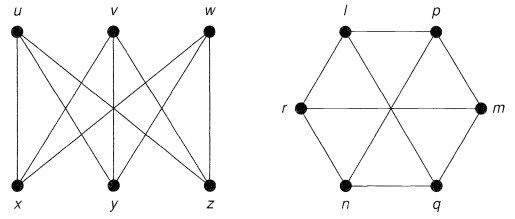
\includegraphics[scale=0.4]{figures/isomorphism1.png}
	\caption{Two simple graphs that are isomorphic to each other}
	\end{figure}
\item A graph is \underline{\emph{\color{magenta} connected}} if it cannot be expressed as the union of two graphs, and \underline{\emph{\color{magenta} disconnected}}.
	\begin{figure}[h!]
	\centering
	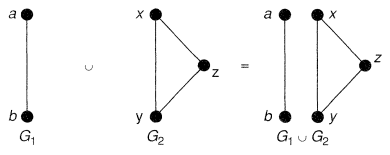
\includegraphics[scale=0.5]{figures/graphUion.png}
	\caption{Each of $G_1$ and $G_2$ is a component of $G_1 \cup G_2$}
	\end{figure}
\item Two vertices $v$ and $w$ of a graph $G$ are \underline{\emph{\color{magenta} adjacent}} if there is an edge $vw$ joining them, and the vertices $v$ and $w$ are then \underline{\emph{\color{magenta} incident}} with such an edge. Similarly, two distinct edges $e$ and $f$ are adjacent if they have a vertex in common.
\item The \underline{\emph{\color{magenta} degree}} of a vertex $v$ of $G$ is the number of edges incident with $v$, and is written $deg(v)$. \emph{Loop}-edge increase node-degree by 2. vertex of degree 0 is an \underline{\emph{\color{magenta} isolated vertex}} and a vertex of degree 1 is an \underline{\emph{\color{magenta} end-vertex}}.
\item \underline{\emph{\color{magenta}Handshaking lemma}}; in any graph the sum of all the vertex-degrees is an even number - in fact, twice the number of edges, since each edge contributes exactly 2 to the sum.
\item A \underline{\emph{\color{magenta}subgraph}} of a graph $G$ is a graph, each of whose vertices belongs to $V(G)$ and each
of whose edges belongs to $E(G)$.
\item \underline{\emph{\color{magenta} Matrix representation}} one way to represent graph is by its \textbf{adjacency matrix} $A$, and its \textbf{incidence matrix} $M$ as follows;
	\begin{figure}[h!]
	\centering
	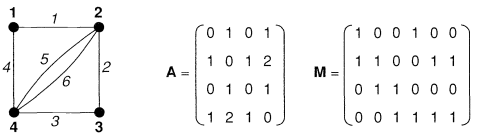
\includegraphics[scale=0.55]{figures/matrixRepresentation.png}
	\end{figure}
\end{itemize}
\newpage
\section*{Exercise 2}
\begin{itemize}
	\item[2a] {\color{blue} Write down the vertex-set and edge-set of each graph in Fig 2.5}
	\begin{figure}[h!]
	\centering
	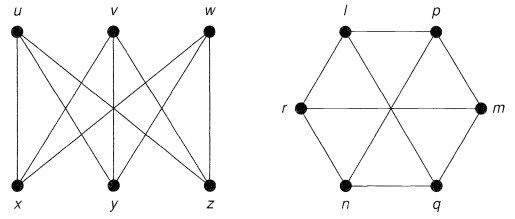
\includegraphics[scale=0.5]{figures/isomorphism1.png}
	\end{figure}
	\hsplit
	
	The first graph $G_1$ is $(V(G_1), E(G_1))$
	\begin{eqnarray*}
	V(G_1) & = & \{ x, y, z, u, v, w\}\\
	E(G_1) & = &	 \{ \{x, u\}, \{x, v\}, \{x, w\}, \\
				  & &    \{y, u\}, \{y, v\}, \{y, w\}, \\ 
				  & &    \{z, u\}, \{z, v\}, \{z, w\} \}
	\end{eqnarray*}
	The second graph $G_2$ is $(V(G_2), E(G_2))$
	\begin{eqnarray*}
	V(G_2) & = & \{ n, m, q, r, l, p\}\\
	E(G_2) & = &	 \{ \{n, r\}, \{n, p\}, \{n, q\}, \\
				  & &    \{m, r\}, \{m, p\}, \{m, q\}, \\ 
				  & &    \{l, r\}, \{l, p\}, \{l, q\} \}
	\end{eqnarray*}
	
	\item[2b] {\color{blue} Draw; \begin{itemize}
			\item[(i)] a simple graph.
			\item[(ii)] a non-simple graph with no loops.
			\item[(iii)] a non-simple graph with no multiple edges, each having 5 vertices each having 5 vertices and 8 edges.
		\end{itemize}}
		\hsplit
		\begin{itemize}
			\item[]
			\begin{figure}[h!]
			\centering 				
			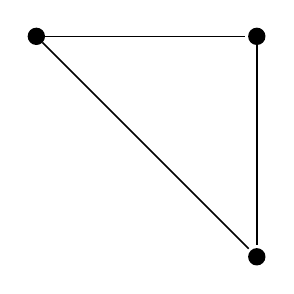
\begin{tikzpicture}[-,>=stealth',shorten >=1pt,auto,node distance=2.8cm,
                    semithick]
 				 \tikzstyle{vert}=[draw, circle, inner sep=2pt,fill]
 					 \node[vert] (A)                    {};
  					 \node[vert]         (B) [right of=A] {};
  					 \node[vert]         (C) [below of=B] {};
 					 \path (A) edge (B)
 					 		 	(B) edge (C)
 					 			(A) edge (C);
				\end{tikzpicture}
				\caption{ (i) a simple graph}
			\end{figure}
		\item[]
			\begin{figure}[h!]
			\centering 				
			\			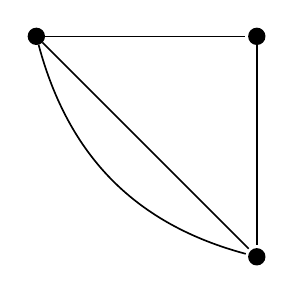
\begin{tikzpicture}[-,>=stealth',shorten >=1pt,auto,node distance=2.8cm,
                    semithick]
 				 \tikzstyle{vert}=[draw, circle, inner sep=2pt,fill]
 					 \node[vert] (A)                    {};
  					 \node[vert]         (B) [right of=A] {};
  					 \node[vert]         (C) [below of=B] {};
 					 \path (A) edge (B)
 					 		 	(B) edge (C)
 					 			(A) edge (C)
 					 			(A) edge [bend right] (C);
				\end{tikzpicture}
				\caption{(ii) a non-simple graph with no loops}
			\end{figure}
		\item[]
			\begin{figure}[h!]
			\centering 				
			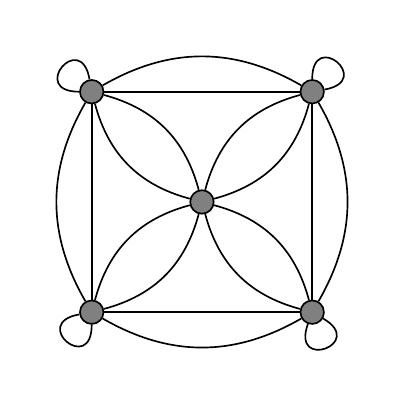
\begin{tikzpicture}[-,auto,node distance=2.8cm,semithick]
 				 \tikzstyle{vert}=[draw, circle, inner sep=3pt,fill=gray]
 					 \node[vert] (A)                    {};
  					 \node[vert]         (B) [right of=A] {};
  					 \node[vert]         (C) [below of=B] {};
  					 \node[vert]         (D) [below of=A] {};
  					 \node[vert]         (E) at ($(D)!0.5!(B)$) {};
 					 \path
 					 			(A) edge (B)
 					 			(A) edge [bend left] (B)
 					 		 	(B) edge (C)
 					 		 	(B) edge [bend left] (C)
 					 			(C) edge (D)
 					 			(C) edge [bend left] (D)
 					 			(A) edge (D)
 					 			(A) edge [bend right] (D)
 					 			(A) edge [bend right] (E)
 					 			(A) edge [bend left] (E)
								(B) edge [bend right] (E)
 					 			(B) edge [bend left] (E)
 					 			(C) edge [bend right] (E)
 					 			(C) edge [bend left] (E)
 					 			(D) edge [bend right] (E)
 					 			(D) edge [bend left] (E);
					\draw[semithick,-] (A) to [out=100, in=180,loop] (A);
					\draw[semithick,-] (B) to [out=10, in=90,loop] (B);
					\draw[semithick,-] (C) to [out=-110, in=-30, loop] (C); 	
					\draw[semithick,-] (D) to [out=-170, in=-90, loop] (D); 					 			 					 			
				\end{tikzpicture}
				\caption{(iii) a 5-vertices and 8-degress each}
			\end{figure}			
		\end{itemize}
	\item[2c] {\color{blue} Draw;
		\begin{itemize}
			\item[(i)] Draw a graph on six vertices whose degrees are 5,5,5,5,3,3; does there exist  a simple graph with these degrees?
			\item[(ii)] How does the answer to part (i) changed if the degrees are 5, 5, 4, 3, 3,2?
		\end{itemize}}
		\hsplit
					\begin{figure}[h!]
			\centering 				
			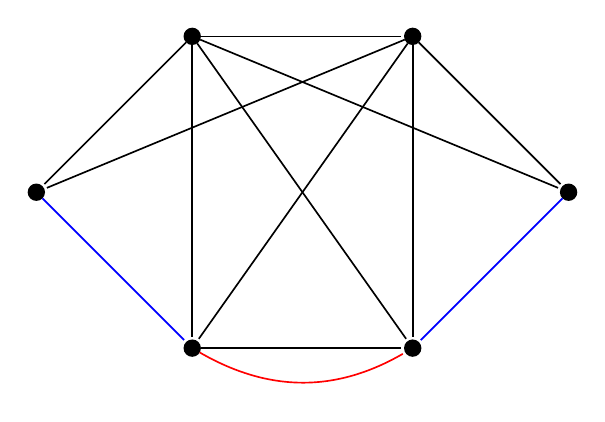
\begin{tikzpicture}[-,>=stealth',shorten >=1pt,auto,node distance=2.8cm, semithick]
 				 \tikzstyle{vert}=[draw, circle, inner sep=2pt,fill]
 					 \node[vert] 			(A)                    {};
  					 \node[vert]         (B) [right of=A] {};
  					 \node[vert]         (C) [below left of=A] {};
  					 \node[vert] 		  (D) [below right of=B] {};
  					 \node[vert]		  (E) [below right of=C] {};
  					 \node[vert]		  (F) [below left of=D] {};
  					
 					  \path
 					  			(A) edge (B)
 					 			(A) edge (C)
 					 			(A) edge (D)
 					 			(A) edge (E)
								(A) edge (F) 					 			
 					 			(B) edge (C)
 					 			(B) edge (D)
 					 			(B) edge (E)
 					 			(B) edge (F)
 					 			(E) edge (F)
								(E) edge [bend right, color=red] (F) 					 			
 					 			(C) edge [color=blue] (E)
 					 			(D) edge [color=blue] (F);
				\end{tikzpicture}
				\caption{(i) a non-simple graph with with 6-vertices with degrees [5,5,5,5,3,3]}
			\end{figure}\\
			There isn't a simple graph with last mentioned degrees for a 6-vertices graph. But it we just remove the red-arc and one of the blue-arcs, we then get a simple graph as shown in the next figure. 
			\begin{figure}[h!]
			\centering 				
			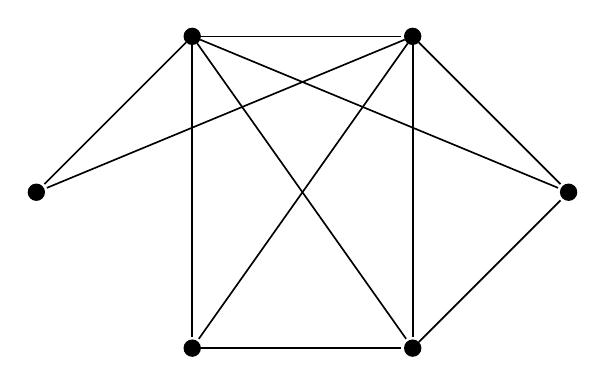
\begin{tikzpicture}[-,>=stealth',shorten >=1pt,auto,node distance=2.8cm, semithick]
 				 \tikzstyle{vert}=[draw, circle, inner sep=2pt,fill]
 					 \node[vert] 			(A)                    {};
  					 \node[vert]         (B) [right of=A] {};
  					 \node[vert]         (C) [below left of=A] {};
  					 \node[vert] 		  (D) [below right of=B] {};
  					 \node[vert]		  (E) [below right of=C] {};
  					 \node[vert]		  (F) [below left of=D] {};
  					
 					  \path
 					  			(A) edge (B)
 					 			(A) edge (C)
 					 			(A) edge (D)
 					 			(A) edge (E)
								(A) edge (F) 					 			
 					 			(B) edge (C)
 					 			(B) edge (D)
 					 			(B) edge (E)
 					 			(B) edge (F)
 					 			(E) edge (F)
 					 			(F) edge (D);
				\end{tikzpicture}
				\caption{(i) a simple graph with with 6-vertices with degrees [5,5,4,3,3,2]}
			\end{figure}\\
\item[(2d)] {\color{blue} Verify that handshaking lemma is hold for figure 2.1}
\hsplit
\begin{figure}[h!]
\centering
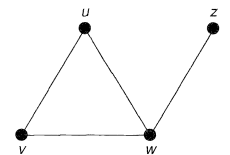
\includegraphics[scale=0.5]{figures/2_d.png}
\end{figure}
As we can see in the last figure, the sum of all vertex-degrees is $2+2+3+1=8$ which is an even number.
\item[(2f)] {\color{blue} \begin{itemize}
	\item[(i)] By suitably lettering the vertices, show that the two graphs in Fig. 2.20 are isomorphic.
	\item[(ii)] Explain why two graphs in Fig. 2.21 are not isomorphic.
\end{itemize}  }
\hsplit
(i) As shown in the following figure \ref{isomorphic} the two graphs are labeled with the same letters in a way to emphasize that they are both isomorphic to each other.
\begin{figure}[h!]
			\centering 				
			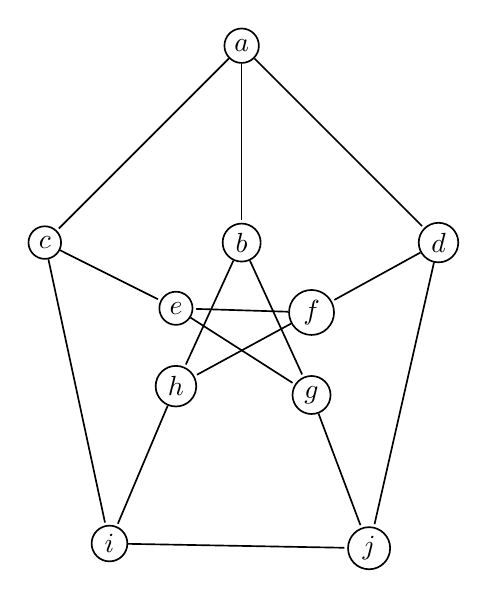
\begin{tikzpicture}[-,>=stealth',shorten >=1pt,auto,node distance=2.5cm, semithick]
 				 \tikzstyle{vert}=[draw, circle, inner sep=2pt,fill=white]
 					 \node[vert] 			(A)                    		{$a$};
  					 \node[vert]         (B) [below of=A] {$b$};
  					 \node[vert]         (C) [left of=B] 		{$c$};
  					 \node[vert]         (D) [right of=B] 	{$d$};
					\node[vert]		  (E) [below left=0.5cm and 0.5cm of B] {$e$};
					\node[vert]		  (F) [below right=0.5cm and 0.5cm of B] {$f$};
					\node[vert]		  (G) [below=0.5cm and 0cm of F] {$g$}; 					 
  					 \node[vert]		  (H) [below= 0.5cm and 0.5cm of E] {$h$};
  					 \node[vert]		  (I)  [below right=3.5cm and 0.5cm of C] {$i$};
  					 \node[vert]		  (J)  [below left=3.5cm and 0.5cm of D] {$j$};
 					  \path
 					  			(A) edge (B)
 					 			(A) edge (C)
 					 			(A) edge (D)
 					 			(B) edge (H)
 					 			(B) edge (G)
 					 			(D) edge (F)
 					 			(F) edge (H)
 					 			(C) edge (E)
 					 			(E) edge (G)
 					 			(C) edge (I)
 					 			(H) edge (I)
 					 			(D) edge (J)
 					 			(G) edge (J)
 					 			(F) edge (E)
 					 			(I) edge (J);
				\end{tikzpicture}
			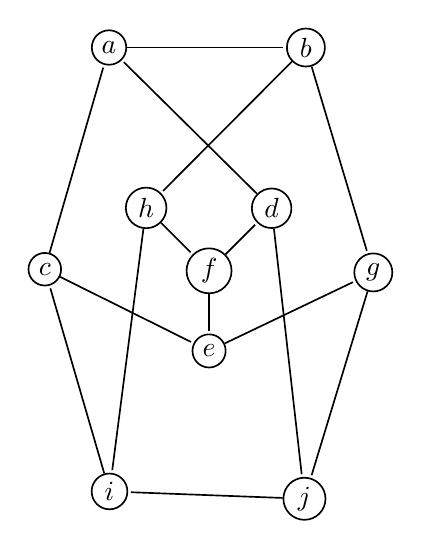
\begin{tikzpicture}[-,>=stealth',shorten >=1pt,auto,node distance=2.5cm, semithick]
 				 \tikzstyle{vert}=[draw, circle, inner sep=2pt,fill=white]
 					 \node[vert] 			(A)                    		{$a$};
  					 \node[vert]         (B) [right of=A] {$b$};
  					 \node[vert]         (C) [below left=2.5cm and 0.5cm of A] 		{$c$};
  					 \node[vert]         (D) [below right=2.5cm and 0.5cm of B] 	{$g$};
					\node[vert]		  (F) at ($(C)!0.5!(D)$) {$f$};
					\node[vert]		  (E) [above left=0.4cm and 0.4cm of F] {$h$};
					\node[vert]		  (G) [above right=0.4cm and 0.4cm of F] {$d$};															
					\node[vert]		  (H) [below=0.5cm and 0cm of F] {$e$}; 					 
  					 \node[vert]		  (I)  [below right=2.5cm and 0.5cm of C] {$i$};
  					 \node[vert]		  (J)  [below left=2.5cm and 0.5cm of D] {$j$};
 					  \path
 					  (A) edge (B)
 					  (B) edge (D)
 					  (D) edge (J)
 					  (J) edge (I)
 					  (I) edge (C)
 					  (C) edge (A)
 					  (C) edge (H)
 					  (H) edge (D)
 					  (B) edge (E)
 					  (E) edge (F)
 					  (F) edge (H)
 					  (F) edge (G)
 					  (G) edge (A)
 					  (G) edge (J)
 					  (E) edge (I);
				\end{tikzpicture}
				\caption{(i) }
				\label{isomorphic}
			\end{figure}\\
(ii) As shown in the following figure \ref{notisomorphic}, we cannot find the red part of the first graph as a subset in the second graph.
\begin{figure}[h!]
\centering
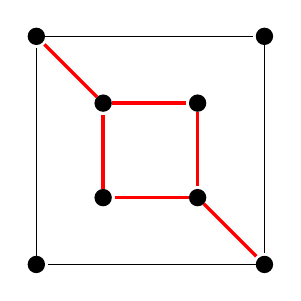
\begin{tikzpicture}[-,>=stealth',shorten >=1pt,auto,node distance=1.2cm, semithick]
 				 \tikzstyle{vert}=[draw, circle, inner sep=2pt,fill]
 					 \node[vert] 			(A)                    		{};
 					 \node[vert] 			(B) [right of=A]                   		{};
 					 \node[vert] 			(C) [below of=B]                   		{};
 					 \node[vert] 			(D) [below of=A]                  		{};
 					 \node[vert]          (E) [above left of=A] {};
 					 \node[vert]          (F) [above right of=B] {};
 					 \node[vert]          (G) [below right of=C] {};
 					 \node[vert]          (H) [below left of=D] {};
				\path
				(A) edge [color=red, very thick] (B)
				(B) edge [color=red, very thick] (C)
				(C) edge [color=red, very thick] (D)
				(D) edge [color=red, very thick] (A)
				(E) edge (F)
				(F) edge (G)
				(G) edge (H)
				(H) edge (E)
				(A) edge [color=red, very thick] (E)
				(C) edge [color=red, very thick] (G);
\end{tikzpicture}
\qquad
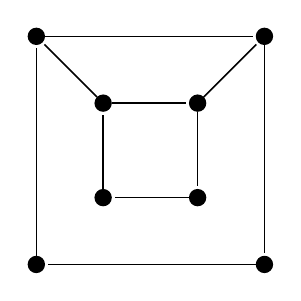
\begin{tikzpicture}[-,>=stealth',shorten >=1pt,auto,node distance=1.2cm, semithick]
 				 \tikzstyle{vert}=[draw, circle, inner sep=2pt,fill]
 					 \node[vert] 			(A)                    		{};
 					 \node[vert] 			(B) [right of=A]                   		{};
 					 \node[vert] 			(C) [below of=B]                   		{};
 					 \node[vert] 			(D) [below of=A]                  		{};
 					 \node[vert]          (E) [above left of=A] {};
 					 \node[vert]          (F) [above right of=B] {};
 					 \node[vert]          (G) [below right of=C] {};
 					 \node[vert]          (H) [below left of=D] {};
				\path
				(A) edge (B)
				(B) edge (C)
				(C) edge (D)
				(D) edge (A)
				(E) edge (F)
				(F) edge (G)
				(G) edge (H)
				(H) edge (E)
				(A) edge (E)
				(B) edge (F);
\end{tikzpicture}
\caption{(ii) not isomorphic graphs}
\label{notisomorphic}
\end{figure}
\end{itemize}
\clearpage 

\section*{3: Examples of graphs}
\begin{itemize}
	\item \underline{\emph{\color{magenta} Null graphs}}, a graph whose edge-set is empty. \underline{\emph{\color{magenta} Complete graph}}, a simple graph in which each pair of distinct vertices are adjacent, in this case $k$-vertex must has $n(n-1)/2$ edges as $n$ the total number of vertices.
	\item \underline{\emph{\color{magenta} Regular graph}}, a graph in which each vertex has the same degree. \textbf{Platonic graphs}, formed from the vertices and edges of the five regular (Platonic) solids - the tetrahedron, octahedron, cube.
	\item \underline{\emph{\color{magenta}Bipartite graph}}, If the vertex set of a graph G can be split into two disjoint sets A and B so that each edge of G joins a vertex of A and a vertex of B.  A \textbf{complete bipartite graph} is a bipartite graph in which each vertex in A is joined to each vertex in B by just one edge.
	\item \underline{\emph{\color{magenta} Cubes}}, the $k$-cube $Q_k$ is the graph whose vertices correspond to the sequences ($a_1, a_2, \cdots, a_k$ ), where each $a_i = 0 $ or $1$, and whose edges join those sequences that differ in just one place. You should check that $Q_k$ has $2^{k}$ vertices and $k 2^{k-1}$ edges, and is regular of degree $k$.\\
	\begin{figure}[h!]
	\centering
	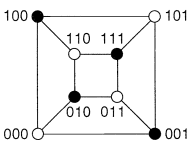
\includegraphics[scale=0.7]{figures/cube1.png}
	\end{figure}
	\item \underline{\emph{\color{magenta}Complement of a simple graph}}, if $G$ is a simple graph with vertex set $V(G)$, its complement $\overline{G}$ is the simple graph with vertex set $V(G)$ in which two vertices are adjacent if and only if they are not adjacent in $G$.
\end{itemize}
\vfill
\section*{Exercise 3}
\begin{itemize}
	\item[(3a)] {\color{blue} Draw the following graphs:
	\begin{itemize}
		\item[(i)] the null graph $N_5$.
		\item[(ii)] the complete graph $K_6$.
		\item[(iii)] the complete bipartite graph $K_{2,4}$.
		\item[(iv)] the union of $K_{1,3}$ and $W_4$.
		\item[(v)] the complement of the cycle graph $C_4$.
\end{itemize}		
	} 
	\hsplit
		\begin{figure}[h!]
	\centering
	\begin{tikzpicture}[-,auto,node distance=2cm, semithick]
 		\tikzstyle{vert}=[draw, circle, inner sep=2pt,fill]
			\node[vert]  (1) {};
			\node[vert]  (2) [right of=1]{};
			\node[vert]  (3) [right of=2]{};		
		 	\node[vert]  (4) [below of=1]{};
		 	\node[vert]  (5) [below of=2]{};
 	\end{tikzpicture}
 	\caption{(i) Null graph $N_5$}
	\end{figure}
	\begin{figure}[h!]
	\centering
	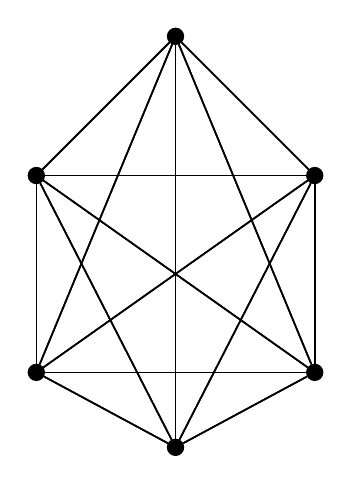
\begin{tikzpicture}[-,auto,node distance=2.5cm, semithick]
 				 \tikzstyle{vert}=[draw, circle, inner sep=2pt,fill]
			\node[vert]  (1) {};
			\node[vert]  (2) [below right of=1]{};
			\node[vert]  (3) [below left of=1]{};		
		 	\node[vert]  (4) [below of=2]{};
		 	\node[vert]  (5) [below of=3]{};
		 	\node[vert]  (6) [below=5cm and 0cm of 1]{};
		
		 		\foreach \i in {1,...,6}{
		 		 \foreach \j in {1,...,6}{
		 			\draw  (\i) -- (\j);
		 			}
		 			}
 	\end{tikzpicture}
 	\caption{(ii) Complete graph $K_6$}
	\end{figure}
		\begin{figure}[h!]
	\centering
	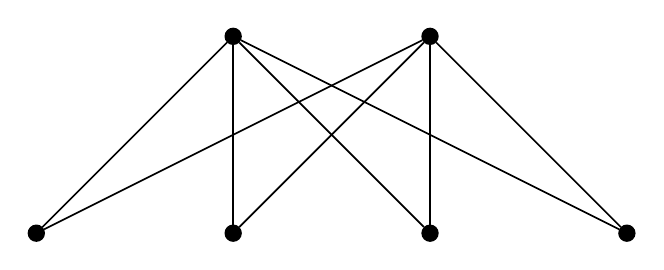
\begin{tikzpicture}[-,auto,node distance=2.5cm, semithick]
 				 \tikzstyle{vert}=[draw, circle, inner sep=2pt,fill]
			\node[vert]  (A) {};
			\node[vert]  (B) [right of=A]{};
			\node[vert]  (2) [below of=A]{};
			\node[vert]  (1) [left of=2]{};		
		 	\node[vert]  (3) [below of=B]{};
		 	\node[vert]  (4) [right of=3]{};
		
		 		\foreach \i in {A,...,B}{
		 		 \foreach \j in {1,...,4}{
		 			\draw  (\i) -- (\j);
		 			}
		 			}
 	\end{tikzpicture}
 	\caption{(iii) Complete bipartite graph $K_{2,4}$}
	\end{figure}
		\begin{figure}[h!]
	\centering
	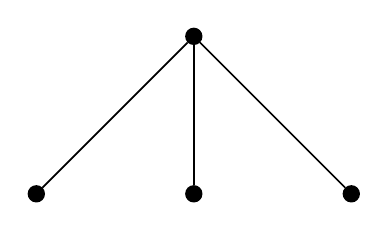
\begin{tikzpicture}[scale=0.8,-,auto,node distance=2cm, semithick]
 				 \tikzstyle{vert}=[draw, circle, inner sep=2pt,fill]
			\node[vert]  (A) {};
			\node[vert]  (2) [below of=A]{};
			\node[vert]  (1) [left of=2]{};		
		 	\node[vert]  (3) [right of=2]{};
		
		 		 \foreach \j in {1,...,3}{
		 			\draw  (A) -- (\j);
		 			}
 	\end{tikzpicture}
 	  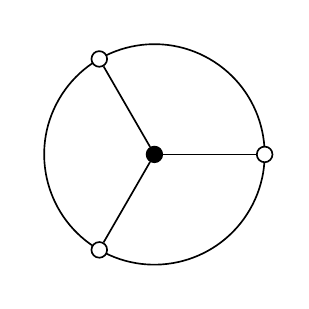
\begin{tikzpicture}[scale=.7, semithick]
 	  \tikzstyle{vert}=[draw, circle, inner sep=2pt,fill]
\draw (60:2) arc (60:420:20mm);
    \node[vert] (center) at (0,0) {};
\foreach \phi in {1,...,3}{
    \node[vert,fill=white] (v_\phi) at (360/3 * \phi:2cm) {};
         \draw (v_\phi) -- (center);
      }
   \end{tikzpicture}
 	\caption{(iv) Union of $K_{1,3}$ and $W_4$}
	\end{figure}
	
	\begin{figure}[h!]
	\centering
	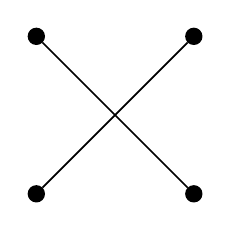
\begin{tikzpicture}[scale=1,-,auto,node distance=2cm, semithick]
 				 \tikzstyle{vert}=[draw, circle, inner sep=2pt,fill]
			\node[vert]  (A) {};
			\node[vert]  (B) [right of=A]{};
			\node[vert]  (C) [below of=B]{};		
		 	\node[vert]  (D) [below of=A]{};
			\path
				(A) edge (C)
				(B) edge (D);
		\end{tikzpicture}
 	\caption{(iv) Complement of cycle graph $C_4$}
	\end{figure}
	\newpage
\item[(3c)] {\color{blue}Draw the graphs $K_{2,2,2}$, and $K_{3,3,2}$, and write down the number of edges of $K_{3,4,5}$}.
\hsplit
The graphs $K_{2,2,2}$ and $K_{3,3,2}$ are shown in the following figures, respectively.\\
For the graph $K_{3,4,5}$, there is 47 edges. 
\begin{figure}[h!]
\centering
	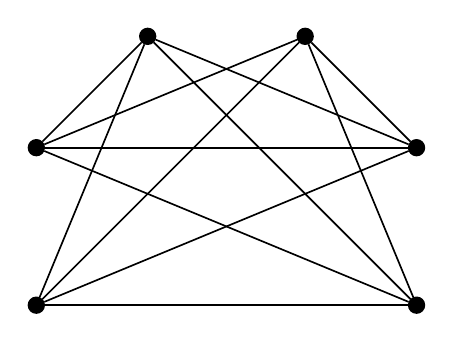
\begin{tikzpicture}[scale=0.6,-,auto,node distance=2cm, semithick]
 				 \tikzstyle{vert}=[draw, circle, inner sep=2pt,fill]
			\node[vert]  (A) {};
			\node[vert]  (B) [right of=A]{};
			\node[vert]  (1) [below left of=A]{};		
		 	\node[vert]  (2) [below of=1]{};
		 	\node[vert] (C) [below  right of=B]{};
		 	\node[vert] (D) [below of=C]{};
			
				\foreach \i in {A,...,D}{
		 		 \foreach \j in {1,...,2}{
		 			\draw  (\i) -- (\j);
		 			}
		 			}
		 		\foreach \i in {A,...,B}{
		 		 \foreach \j in {C,...,D}{
		 			\draw  (\i) -- (\j);
		 			}
		 			}
 	\end{tikzpicture}
 	\caption{$K_{2,2,2}$}
\end{figure}
\begin{figure}[h!]
\centering
	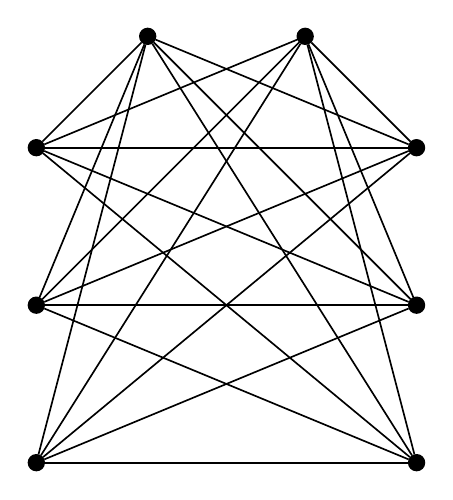
\begin{tikzpicture}[scale=0.6,-,auto,node distance=2cm, semithick]
 		\tikzstyle{vert}=[draw, circle, inner sep=2pt,fill]
			\node[vert]  (A) {};
			\node[vert]  (B) [right of=A]{};			
			\node[vert]  (1) [below left of=A]{};		
		 	\node[vert]  (2) [below of=1]{};
		 	\node[vert] (3) [below of=2] {};
		 	\node[vert] (C) [below  right of=B]{};
		 	\node[vert] (D) [below of=C]{};
		 	\node[vert] (E) [below of=D]{};
			
				\foreach \i in {A,...,E}{
		 		 \foreach \j in {1,...,3}{
		 			\draw  (\i) -- (\j);
		 			}
		 			}
		 		\foreach \i in {A,...,B}{
		 		 \foreach \j in {C,...,E}{
		 			\draw  (\i) -- (\j);
		 			}
		 			}
 	\end{tikzpicture}
 	\caption{$K_{3,3,2}$}
\end{figure}
\item[(3g)] {\color{blue} A simple graph that is isomorphic to its complement is self-complementary.
	\begin{itemize}
		\item[(i)] Prove that, if $G$ is self-complementary, then $G$ has $4k$ or $4k+1$ vertices, where $k$ is an integer,
		\item[(ii)] Find all self-complementary graphs with 4 and 5 vertices,
		\item[(iii)] Find a self-complementary graph with 8 vertices.
	\end{itemize}}
	\hsplit
	\begin{itemize}
		\item[(i)] \underline{Proof}\\
			If $G$ is a self-complementary with $n$ vertices, and $$ G \cup \overline{G} =  K_n.$$ But we know that, the total number of edge in the complete graph $K_n$ i.e. $|E(K_n)| $is $n(n-1)/2$, that is, $$|E(G)| =  |E(\overline{G})| = \frac{n(n-1)}{4}.$$ In other words, $n$ or $n-1$ must be divisible by 4, that is, when $n$ is $4k$ or $4k+1$.
			\item[]
			\begin{figure}[h!]
			\centering
				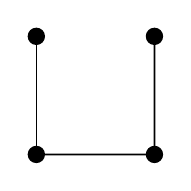
\begin{tikzpicture}[scale=0.4,-,auto,node distance=1.5cm, semithick]
 				 \tikzstyle{vert}=[draw, circle, inner sep=2pt,fill]
						\node[vert]  (A) {};
						\node[vert] (B) [below of=A]{};
						\node[vert] (C) [right of=B]{};
						\node[vert] (D) [above of=C]{};
						
						\path
							(A) edge (B)
							(B) edge (C)
							(C) edge (D);
 				\end{tikzpicture}
				\qquad	
 				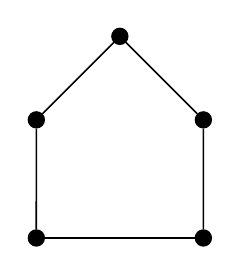
\begin{tikzpicture}[scale=0.4,-,auto,node distance=1.5cm, semithick]
 				 \tikzstyle{vert}=[draw, circle, inner sep=2pt,fill]
						\node[vert]  (A) {};
						\node[vert] (B) [below left of=A]{};
						\node[vert] (C) [below right of=A]{};
						\node[vert] (D) [below of=B]{};
						\node[vert] (E) [below of=C]{};
						
						\path
							(A) edge (B)
							(A) edge (C)
							(B) edge (D)
							(C) edge (E)
							(D) edge (E);
 				\end{tikzpicture}
				\qquad	
 				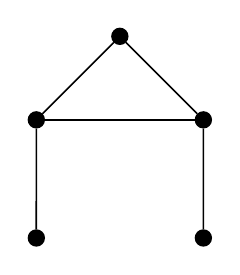
\begin{tikzpicture}[scale=0.4,-,auto,node distance=1.5cm, semithick]
 				 \tikzstyle{vert}=[draw, circle, inner sep=2pt,fill]
						\node[vert]  (A) {};
						\node[vert] (B) [below left of=A]{};
						\node[vert] (C) [below right of=A]{};
						\node[vert] (D) [below of=B]{};
						\node[vert] (E) [below of=C]{};
						
						\path
							(A) edge (B)
							(A) edge (C)
							(B) edge (D)
							(C) edge (E)
							(B) edge (C);
			
 				\end{tikzpicture}
				\caption{(ii) 4 and 5 vertices self-complementary graphs}
			\end{figure}
			\begin{figure}[h!]
			\centering
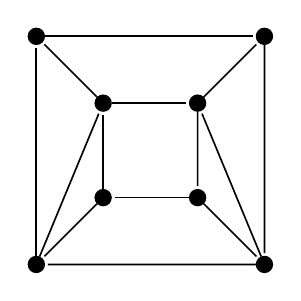
\begin{tikzpicture}[scale=.8,-,>=stealth',shorten >=1pt,auto,node distance=1.2cm, semithick]
 				 \tikzstyle{vert}=[draw, circle, inner sep=2pt,fill]
 					 \node[vert] 			(A)                    		{};
 					 \node[vert] 			(B) [right of=A]                   		{};
 					 \node[vert] 			(C) [below of=B]                   		{};
 					 \node[vert] 			(D) [below of=A]                  		{};
 					 \node[vert]          (E) [above left of=A] {};
 					 \node[vert]          (F) [above right of=B] {};
 					 \node[vert]          (G) [below right of=C] {};
 					 \node[vert]          (H) [below left of=D] {};
				\path
				(A) edge (B)
				(B) edge (C)
				(C) edge (D)
				(D) edge (A)
				(E) edge (F)
				(F) edge (G)
				(G) edge (H)
				(H) edge (E)
				(A) edge (E)
				(B) edge (F)
				(C) edge (G)
				(D) edge (H)
				(G) edge (B)
				(H) edge (A);
\end{tikzpicture}
\caption{(iii) a self-complementary graph with 8 vertices}
			\end{figure}
	\end{itemize}
\end{itemize}
\section*{4: Embeddings of graphs}
\begin{itemize}
		\item \underline{\emph{\color{magenta} Jordan curve}} is a continuous curve which doesn't intersect itself.
		\item \underline{\emph{\color{magenta} Graph embedding}}: A graph $G$ can be embedded (or has an embedding) in a given space if it is isomorphic to a graph drawn in the space with points representing vertices of $G$ and Jordan curves representing edges in such a way that there are no crossings.
		\item \underline{\emph{\color{magenta} Theorem 4A}}: \hl{\emph{Every graph can be embedded in Euclidean 3-space}}.
		\item \underline{\emph{\color{magenta} Planer graph}}: a graph that can be embedded in a plane.
		\item \underline{\emph{\color{magenta} Theorem 4B}}:\hl{\emph{A graph is planer if and only if it can be embedded on the surface of a sphere}}.
\end{itemize}

\section*{5: More definitions}
\begin{itemize}
		\item A \underline{\emph{\color{magenta} walk}} in $G$ is a finite sequence of edges of the form $v_0 v_1, v_1 v_2, \cdots, v_{m-1} v_m$, where $v_0$ is the \textbf{initial vertex} and $v_m$ is the \textbf{finial vertex} of the walk, also the number of edges is called \textbf{length}.
		\item \underline{\emph{\color{magenta} Trial}} is a walk in which all the edges are distinct. \underline{\emph{\color{magenta} path}} is a trial with all vertices are distinct also (expect, possibly $v_0 = v_m$ where then we call the trial or the path \underline{\emph{\color{magenta} closed}}). A closed path containing at least one edge is a \underline{\emph{\color{magenta} cycle}}\footnote{called \emph{circuit} in 3rd edition of the textbook}.
		\item A graph is \underline{\emph{\color{magenta} connected}} if and only if there is a path between each pair of vertices.
		\item \underline{\emph{\color{magenta} Theorem 5.1}} \hl{\emph{If $G$ is a bipartite graph, then each of $G$ has even length}}.
		\item \underline{\emph{\color{magenta} Theorem 5.2}} \hl{\emph{Let $G$ be a simple graph on $n$ vertices. If $G$ has $k$ components, then the number $m$ of edges of $G$ satisfies}}
				\begin{equation}
						n-k \leq m \leq (n-k)(n-k+1)/2.
				\end{equation}
		\item \underline{\emph{\color{magenta} Corollary 5.3}} \emph{Any simple graph with $n$ vertices and more than $(n-1)(n-2)/2$ edges is connected}.
		\item A \underline{\emph{\color{magenta} disconnecting set}} in a connected graph $G$ is a set of edges whose removal disconnects $G$ and increases the number of components of $G$.
		\item A \underline{\emph{\color{magenta} cutset}} is defined to be a disconnecting set, no proper subset of which is a disconnecting set. If a cutset has only one edge $e$, we call $e$ a \underline{\emph{\color{magenta} bridge}}.
		\item If $G$ is connected, its \underline{\emph{\color{magenta} edge connectivity}} $\lambda (G)$ is the size of the smallest cutset in $G$. Thus $\lambda (G)$ is the minimum number of edges that we need to delete in order to disconnect $G$.
		\item If $G$ is connected and not a complete graph, its \underline{\emph{\color{magenta} vertex connectivity}} $\mathcal{K}(G)$ is the size of the smallest separating set in $G$. Thus $\mathcal{K}(G)$ is the minimum number of vertices that we need to delete in order to disconnect $G$.
\end{itemize}
\clearpage
\section*{Exercise 5}
\begin{itemize}
		\item[(5a)] {\color{blue} In the Petersen graph, find
						\begin{itemize}
								\item[(i)] a trail of length 5;
								\item[(ii)] a path of length 9;
								\item[(iii)] cycles of lengths 5, 6, 8 and 9;
								\item[(iv)] cutsets with 3, 4 and 5 edges.
						\end{itemize}
				}
				\hsplit
			\begin{figure}[h!]
			\centering 				
			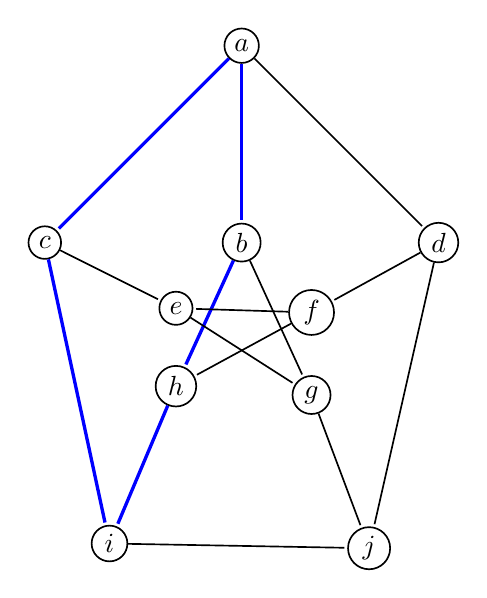
\begin{tikzpicture}[-,>=stealth',shorten >=1pt,auto,node distance=2.5cm, semithick]
 				 \tikzstyle{vert}=[draw, circle, inner sep=2pt,fill=white]
 					 \node[vert] 			(A)                    		{$a$};
  					 \node[vert]         (B) [below of=A] {$b$};
  					 \node[vert]         (C) [left of=B] 		{$c$};
  					 \node[vert]         (D) [right of=B] 	{$d$};
					\node[vert]		  (E) [below left=0.5cm and 0.5cm of B] {$e$};
					\node[vert]		  (F) [below right=0.5cm and 0.5cm of B] {$f$};
					\node[vert]		  (G) [below=0.5cm and 0cm of F] {$g$}; 					 
  					 \node[vert]		  (H) [below= 0.5cm and 0.5cm of E] {$h$};
  					 \node[vert]		  (I)  [below right=3.5cm and 0.5cm of C] {$i$};
  					 \node[vert]		  (J)  [below left=3.5cm and 0.5cm of D] {$j$};
 					  \path
							  (A) edge[color=blue, very thick] (B)
 					 			(A) edge [color=blue, very thick] (C)
 					 			(A) edge (D)
 					 			(B) edge [color=blue, very thick] (H)
 					 			(B) edge (G)
 					 			(D) edge (F)
 					 			(F) edge (H)
 					 			(C) edge (E)
 					 			(E) edge (G)
 					 			(C) edge [color=blue, very thick] (I)
 					 			(H) edge [color=blue, very thick] (I)
 					 			(D) edge (J)
 					 			(G) edge (J)
 					 			(F) edge (E)
 					 			(I) edge (J);
				\end{tikzpicture}
				\caption{(i) a Petersen graph with trail of length 5 highlighted $\{ab, bh, hi, ic, ca\}$}
			\end{figure}
			
			\begin{figure}[h!]
			\centering 				
			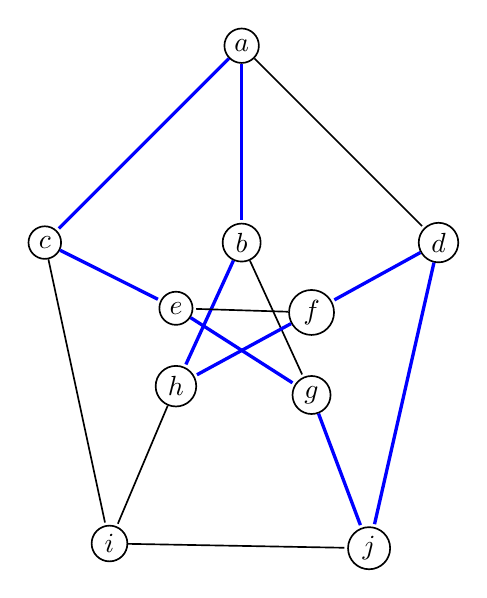
\begin{tikzpicture}[-,>=stealth',shorten >=1pt,auto,node distance=2.5cm, semithick]
 				 \tikzstyle{vert}=[draw, circle, inner sep=2pt,fill=white]
 					 \node[vert] 			(A)                    		{$a$};
  					 \node[vert]         (B) [below of=A] {$b$};
  					 \node[vert]         (C) [left of=B] 		{$c$};
  					 \node[vert]         (D) [right of=B] 	{$d$};
					\node[vert]		  (E) [below left=0.5cm and 0.5cm of B] {$e$};
					\node[vert]		  (F) [below right=0.5cm and 0.5cm of B] {$f$};
					\node[vert]		  (G) [below=0.5cm and 0cm of F] {$g$}; 					 
  					 \node[vert]		  (H) [below= 0.5cm and 0.5cm of E] {$h$};
  					 \node[vert]		  (I)  [below right=3.5cm and 0.5cm of C] {$i$};
  					 \node[vert]		  (J)  [below left=3.5cm and 0.5cm of D] {$j$};
 					  \path
							  (A) edge[color=blue, very thick] (B)
							  (A) edge [color=blue, very thick] (C)
 					 			(A) edge (D)
 					 			(B) edge [color=blue, very thick] (H)
 					 			(B) edge (G)
 					 			(D) edge  [color=blue, very thick] (F)
 					 			(F) edge  [color=blue, very thick] (H)
 					 			(C) edge  [color=blue, very thick] (E)
 					 			(E) edge  [color=blue, very thick] (G)
 					 			(C) edge  (I)
 					 			(H) edge (I)
 					 			(D) edge  [color=blue, very thick] (J)
 					 			(G) edge  [color=blue, very thick] (J)
 					 			(F) edge (E)
 					 			(I) edge (J);
				\end{tikzpicture}
				\caption{(ii) a Petersen graph with path of length 9 highlighted $\{ab, bh, hf, fd, dj, ig, ge, ec, ca \}$}
			\end{figure}
			
			\begin{figure}[h!]
			\centering 				
			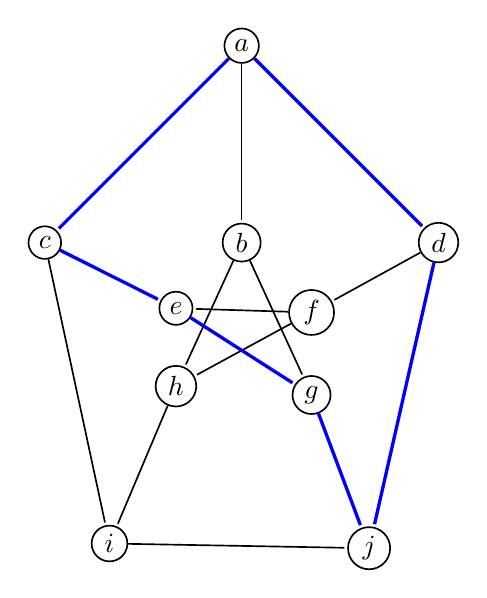
\begin{tikzpicture}[-,>=stealth',shorten >=1pt,auto,node distance=2.5cm, semithick]
 				 \tikzstyle{vert}=[draw, circle, inner sep=2pt,fill=white]
 					 \node[vert] 			(A)                    		{$a$};
  					 \node[vert]         (B) [below of=A] {$b$};
  					 \node[vert]         (C) [left of=B] 		{$c$};
  					 \node[vert]         (D) [right of=B] 	{$d$};
					\node[vert]		  (E) [below left=0.5cm and 0.5cm of B] {$e$};
					\node[vert]		  (F) [below right=0.5cm and 0.5cm of B] {$f$};
					\node[vert]		  (G) [below=0.5cm and 0cm of F] {$g$}; 					 
  					 \node[vert]		  (H) [below= 0.5cm and 0.5cm of E] {$h$};
  					 \node[vert]		  (I)  [below right=3.5cm and 0.5cm of C] {$i$};
  					 \node[vert]		  (J)  [below left=3.5cm and 0.5cm of D] {$j$};
 					  \path
							  (A) edge (B)
 					 			(A) edge [color=blue, very thick] (C)
 					 			(A) edge [color=blue, very thick](D)
 					 			(B) edge  (H)
 					 			(B) edge (G)
 					 			(D) edge (F)
 					 			(F) edge (H)
 					 			(C) edge [color=blue, very thick](E)
 					 			(E) edge [color=blue, very thick](G)
 					 			(C) edge  (I)
 					 			(H) edge  (I)
 					 			(D) edge [color=blue, very thick](J)
 					 			(G) edge [color=blue, very thick](J)
 					 			(F) edge (E)
 					 			(I) edge (J);
				\end{tikzpicture}
				\caption{While (i) also represents a cycle of 5 length, this represents a cycle of 6 length highlighted $\{ac, ce, eg, gj, jd, da\}$}
			\end{figure}

			\begin{figure}[h!]
			\centering 				
			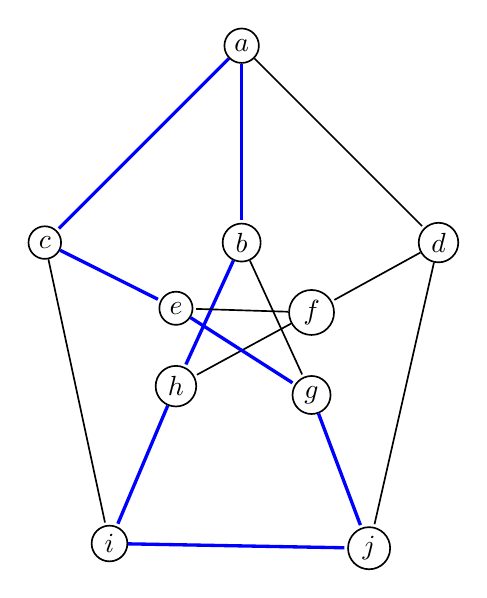
\begin{tikzpicture}[-,>=stealth',shorten >=1pt,auto,node distance=2.5cm, semithick]
 				 \tikzstyle{vert}=[draw, circle, inner sep=2pt,fill=white]
 					 \node[vert] 			(A)                    		{$a$};
  					 \node[vert]         (B) [below of=A] {$b$};
  					 \node[vert]         (C) [left of=B] 		{$c$};
  					 \node[vert]         (D) [right of=B] 	{$d$};
					\node[vert]		  (E) [below left=0.5cm and 0.5cm of B] {$e$};
					\node[vert]		  (F) [below right=0.5cm and 0.5cm of B] {$f$};
					\node[vert]		  (G) [below=0.5cm and 0cm of F] {$g$}; 					 
  					 \node[vert]		  (H) [below= 0.5cm and 0.5cm of E] {$h$};
  					 \node[vert]		  (I)  [below right=3.5cm and 0.5cm of C] {$i$};
  					 \node[vert]		  (J)  [below left=3.5cm and 0.5cm of D] {$j$};
 					  \path
							  (A) edge [color=blue, very thick](B)
 					 			(A) edge [color=blue, very thick] (C)
 					 			(A) edge (D)
 					 			(B) edge  [color=blue, very thick](H)
 					 			(B) edge (G)
 					 			(D) edge (F)
 					 			(F) edge (H)
 					 			(C) edge [color=blue, very thick](E)
 					 			(E) edge [color=blue, very thick](G)
 					 			(C) edge  (I)
 					 			(H) edge  [color=blue, very thick](I)
 					 			(D) edge (J)
 					 			(G) edge [color=blue, very thick](J)
 					 			(F) edge (E)
 					 			(I) edge [color=blue, very thick](J);
				\end{tikzpicture}
				\caption{A cycle of 8 length highlighted $\{ac, ce, eg, gj, ji, ih, hb, ba\}$}
			\end{figure}

			\begin{figure}[h!]
			\centering 				
			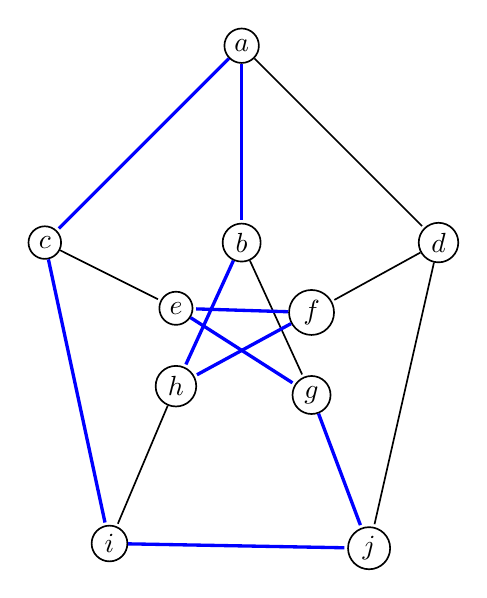
\begin{tikzpicture}[-,>=stealth',shorten >=1pt,auto,node distance=2.5cm, semithick]
 				 \tikzstyle{vert}=[draw, circle, inner sep=2pt,fill=white]
 					 \node[vert] 			(A)                    		{$a$};
  					 \node[vert]         (B) [below of=A] {$b$};
  					 \node[vert]         (C) [left of=B] 		{$c$};
  					 \node[vert]         (D) [right of=B] 	{$d$};
					\node[vert]		  (E) [below left=0.5cm and 0.5cm of B] {$e$};
					\node[vert]		  (F) [below right=0.5cm and 0.5cm of B] {$f$};
					\node[vert]		  (G) [below=0.5cm and 0cm of F] {$g$}; 					 
  					 \node[vert]		  (H) [below= 0.5cm and 0.5cm of E] {$h$};
  					 \node[vert]		  (I)  [below right=3.5cm and 0.5cm of C] {$i$};
  					 \node[vert]		  (J)  [below left=3.5cm and 0.5cm of D] {$j$};
 					  \path
							  (A) edge [color=blue, very thick](B)
 					 			(A) edge [color=blue, very thick] (C)
 					 			(A) edge (D)
 					 			(B) edge  [color=blue, very thick](H)
 					 			(B) edge (G)
 					 			(D) edge (F)
 					 			(F) edge [color=blue, very thick](H)
 					 			(C) edge (E)
 					 			(E) edge [color=blue, very thick](G)
 					 			(C) edge  [color=blue, very thick](I)
 					 			(H) edge  (I)
 					 			(D) edge (J)
 					 			(G) edge [color=blue, very thick](J)
 					 			(F) edge [color=blue, very thick](E)
 					 			(I) edge [color=blue, very thick](J);
				\end{tikzpicture}
				\caption{A cycle of 9 length highlighted $\{ac, ci, ij, jg, ge, ef, fh, hb, ba\}$}
			\end{figure}

			\begin{figure}[h!]
			\centering 				
			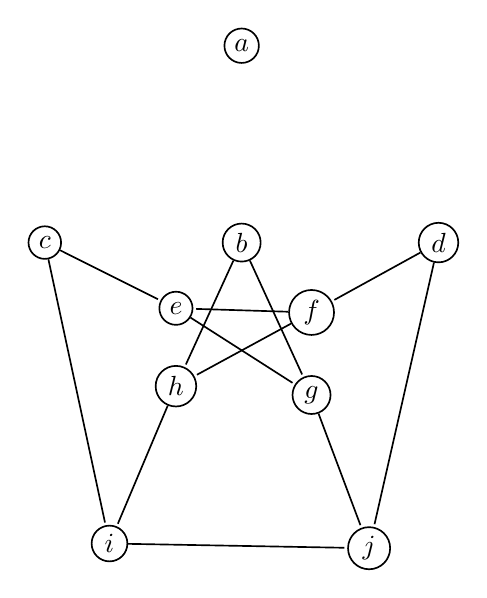
\begin{tikzpicture}[-,>=stealth',shorten >=1pt,auto,node distance=2.5cm, semithick]
 				 \tikzstyle{vert}=[draw, circle, inner sep=2pt,fill=white]
 					 \node[vert] 			(A)                    		{$a$};
  					 \node[vert]         (B) [below of=A] {$b$};
  					 \node[vert]         (C) [left of=B] 		{$c$};
  					 \node[vert]         (D) [right of=B] 	{$d$};
					\node[vert]		  (E) [below left=0.5cm and 0.5cm of B] {$e$};
					\node[vert]		  (F) [below right=0.5cm and 0.5cm of B] {$f$};
					\node[vert]		  (G) [below=0.5cm and 0cm of F] {$g$}; 					 
  					 \node[vert]		  (H) [below= 0.5cm and 0.5cm of E] {$h$};
  					 \node[vert]		  (I)  [below right=3.5cm and 0.5cm of C] {$i$};
  					 \node[vert]		  (J)  [below left=3.5cm and 0.5cm of D] {$j$};
 					  \path
							  %(A) edge (B)
 					 			%(A) edge  (C)	
							  %(A) edge (D)
 					 			(B) edge  (H)
 					 			(B) edge (G)
 					 			(D) edge (F)
 					 			(F) edge (H)
 					 			(C) edge (E)
 					 			(E) edge (G)
 					 			(C) edge  (I)
 					 			(H) edge  (I)
 					 			(D) edge (J)
 					 			(G) edge (J)
 					 			(F) edge (E)
 					 			(I) edge (J);
				\end{tikzpicture}
				\caption{A cutset of 3 edges $\{ac, ab, ac\}$}
			\end{figure}

			\begin{figure}[h!]
			\centering 				
			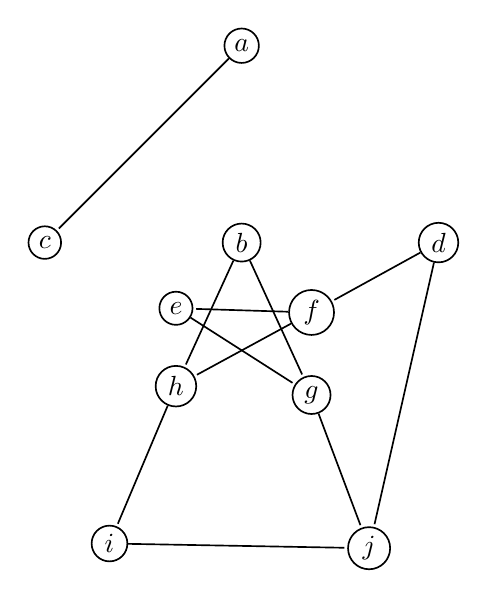
\begin{tikzpicture}[-,>=stealth',shorten >=1pt,auto,node distance=2.5cm, semithick]
 				 \tikzstyle{vert}=[draw, circle, inner sep=2pt,fill=white]
 					 \node[vert] 			(A)                    		{$a$};
  					 \node[vert]         (B) [below of=A] {$b$};
  					 \node[vert]         (C) [left of=B] 		{$c$};
  					 \node[vert]         (D) [right of=B] 	{$d$};
					\node[vert]		  (E) [below left=0.5cm and 0.5cm of B] {$e$};
					\node[vert]		  (F) [below right=0.5cm and 0.5cm of B] {$f$};
					\node[vert]		  (G) [below=0.5cm and 0cm of F] {$g$}; 					 
  					 \node[vert]		  (H) [below= 0.5cm and 0.5cm of E] {$h$};
  					 \node[vert]		  (I)  [below right=3.5cm and 0.5cm of C] {$i$};
  					 \node[vert]		  (J)  [below left=3.5cm and 0.5cm of D] {$j$};
 					  \path
							  %(A) edge (B)
 					 			(A) edge  (C)	
							  %(A) edge (D)
 					 			(B) edge  (H)
 					 			(B) edge (G)
 					 			(D) edge (F)
 					 			(F) edge (H)
 					 			%(C) edge (E)
 					 			(E) edge (G)
 					 			%(C) edge  (I)
 					 			(H) edge  (I)
 					 			(D) edge (J)
 					 			(G) edge (J)
 					 			(F) edge (E)
 					 			(I) edge (J);
				\end{tikzpicture}
				\caption{A cutset of 4 edges $\{ab, ac, ce, ci\}$}
			\end{figure}
			
			\begin{figure}[h!]
			\centering 				
			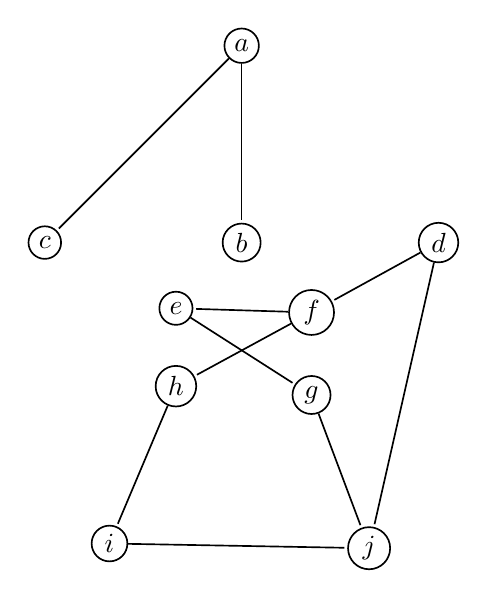
\begin{tikzpicture}[-,>=stealth',shorten >=1pt,auto,node distance=2.5cm, semithick]
 				 \tikzstyle{vert}=[draw, circle, inner sep=2pt,fill=white]
 					 \node[vert] 			(A)                    		{$a$};
  					 \node[vert]         (B) [below of=A] {$b$};
  					 \node[vert]         (C) [left of=B] 		{$c$};
  					 \node[vert]         (D) [right of=B] 	{$d$};
					\node[vert]		  (E) [below left=0.5cm and 0.5cm of B] {$e$};
					\node[vert]		  (F) [below right=0.5cm and 0.5cm of B] {$f$};
					\node[vert]		  (G) [below=0.5cm and 0cm of F] {$g$}; 					 
  					 \node[vert]		  (H) [below= 0.5cm and 0.5cm of E] {$h$};
  					 \node[vert]		  (I)  [below right=3.5cm and 0.5cm of C] {$i$};
  					 \node[vert]		  (J)  [below left=3.5cm and 0.5cm of D] {$j$};
 					  \path
							  	(A) edge (B)
 					 			(A) edge  (C)	
							  	%(A) edge (D)
 					 			%(B) edge  (H)
 					 			%(B) edge (G)
 					 			(D) edge (F)
 					 			(F) edge (H)
 					 			%(C) edge (E)
 					 			(E) edge (G)
 					 			%(C) edge  (I)
 					 			(H) edge  (I)
 					 			(D) edge (J)
 					 			(G) edge (J)
 					 			(F) edge (E)
 					 			(I) edge (J);
				\end{tikzpicture}
				\caption{A cutset of 5 edges $\{ad, bh, bg, ce, ci\}$}
			\end{figure}
			
			\clearpage
	\item[(5c)] {\color{blue}Find $\mathcal{K}(G)$ and $\lambda(G)$ for each of the following graphs (i) $C_6$, (ii) $W_6$, (iii) $K_{4,7}$, (iv) $Q_4$}
	\hsplit
	\begin{figure}[h!]
	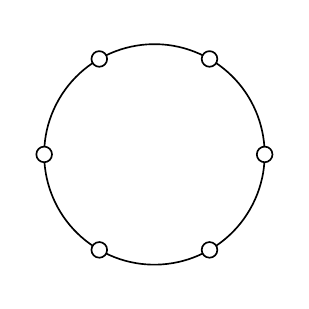
\begin{tikzpicture}[scale=.7, semithick]
 	  \tikzstyle{vert}=[draw, circle, inner sep=2pt,fill]
\draw (60:2) arc (60:420:20mm);
    %\node[vert] (center) at (0,0) {};
\foreach \phi in {1,...,6}{
    \node[vert,fill=white] (v_\phi) at (360/6 * \phi:2cm) {};
         %\draw (v_\phi) -- (center);
      }
   \end{tikzpicture}
   \caption{(i) $\mathcal{K}{(C_6)} = 2$ and $\lambda(C_6) = 2$}
	\end{figure}

	\begin{figure}[h!]
	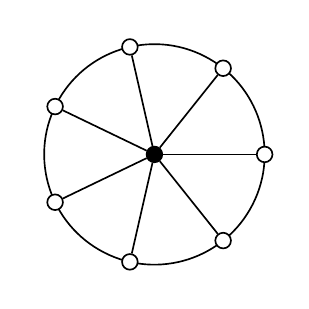
\begin{tikzpicture}[scale=.7, semithick]
 	  \tikzstyle{vert}=[draw, circle, inner sep=2pt,fill]
\draw (60:2) arc (60:420:20mm);
    \node[vert] (center) at (0,0) {};
\foreach \phi in {1,...,7}{
    \node[vert,fill=white] (v_\phi) at (360/7 * \phi:2cm) {};
         \draw (v_\phi) -- (center);
      }
   \end{tikzpicture}
   \caption{(ii) $\mathcal{K}{(W_8)} = 4$ and $\lambda(W_8) = 3$}
	\end{figure}

	\begin{figure}[h!]
	\centering
	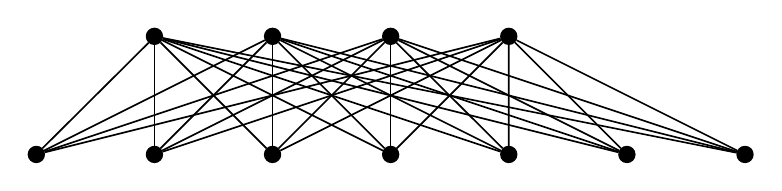
\begin{tikzpicture}[scale=.7,-,auto,node distance=1.5cm, semithick]
 				 \tikzstyle{vert}=[draw, circle, inner sep=2pt,fill]
			\node[vert]  (B) {};
			\node[vert]  (A) [left of=B]{};
			\node[vert]  (C) [right of=B]{};
			\node[vert]  (D) [right of=C]{};
		 	\node[vert]  (3) [below of=B]{};
			\node[vert]  (2) [left of=3]{};		
			\node[vert]  (1) [left of=2]{};
		 	\node[vert]  (4) [right of=3]{};
		 	\node[vert]  (5) [right of=4]{};
		 	\node[vert]  (6) [right of=5]{};
		 	\node[vert]  (7) [right of=6]{};
		
		 		\foreach \i in {A,...,D}{
		 		 \foreach \j in {1,...,7}{
		 			\draw  (\i) -- (\j);
		 			}
		 			}
 	\end{tikzpicture}
	\caption{(iii) $\mathcal{K}{(K_{4,7})} = 4$ and $\lambda(W_8) = 4$}
	\end{figure}
	
	\begin{figure}[h!]
	\centering
	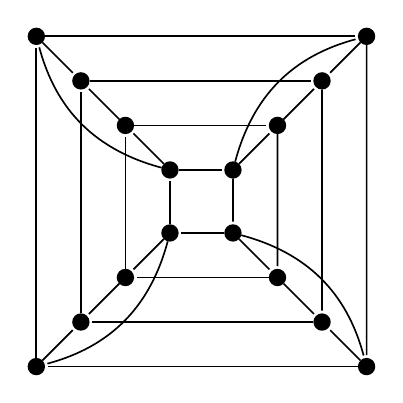
\begin{tikzpicture}[scale=.3,-,>=stealth',shorten >=1pt,auto,node distance=.8cm, semithick]
			\tikzstyle{vert}=[draw, circle, inner sep=2pt,fill]
 					 \node[vert] 			(A)                    		{};
 					 \node[vert] 			(B) [right of=A]                   		{};
 					 \node[vert] 			(C) [below of=B]                   		{};
 					 \node[vert] 			(D) [below of=A]                  		{};
 					 \node[vert]          (E) [above left of=A] {};
 					 \node[vert]          (F) [above right of=B] {};
 					 \node[vert]          (G) [below right of=C] {};
 					 \node[vert]          (H) [below left of=D] {};
					 \node[vert]          (I) [above left of=E] {};
 					 \node[vert]          (J) [above right of=F] {};
 					 \node[vert]          (K) [below right of=G] {};
 					 \node[vert]          (L) [below left of=H] {};
					 \node[vert]          (M) [above left of=I] {};
 					 \node[vert]          (N) [above right of=J] {};
 					 \node[vert]          (O) [below right of=K] {};
 					 \node[vert]          (P) [below left of=L] {};


					 \path
				(A) edge (B)
				(B) edge (C)
				(C) edge (D)
				(D) edge (A)
				(E) edge (F)
				(F) edge (G)
				(G) edge (H)
				(H) edge (E)
				(A) edge (E)
				(B) edge (F)
				(C) edge (G)
				(D) edge (H)
				(I) edge (J)
				(J) edge (K)
				(K) edge (L)
				(L) edge (I)
				(M) edge (N)
				(N) edge (O)
				(O) edge (P)
				(P) edge (M)
				(E) edge (I)
				(F) edge (J)
				(G) edge (K)
				(H) edge (L)
				(M) edge (I)
				(N) edge (J)
				(O) edge (K)
				(P) edge (L)
				(A) edge [bend left] (M)
				(B) edge [bend left] (N)
				(C) edge [bend left] (O)
				(D) edge [bend left] (P)
				;
				
	\end{tikzpicture}
	\caption{(iv) $\mathcal{K}{(Q_{4})} = 3$ and $\lambda(Q_4) = 8$}
	\label{fig_5c_cube}
	\end{figure}
	%\clearpage

	\item[(5f)] {\color{blue} Prove that if $G$ is a simple graph, then $G$ and $\overline{G}$ cannot both be disconnected}
	\hsplit

	To prove this we need to prove that the complement of a disconnected graph $G$ is connected.\\
	That is without loss of generality, assume $G$ is disconnected. Now consider two vertices $x$ and $y$ in $\overline{G}$. If $x$ and $y$ are not adjacent in $G$, then they will be adjacent in $\overline{G}$ and we can find a trivial $x-y$ path. If $x$ and $y$ are adjacent in $G$ then they must have been in the same component. This means that the edges $xz$ and $yz$ were not in $G$. This implies that they both must be edges in $\overline{G}$. This gives us the path $x \rightarrow y \rightarrow z$. Therefore, in $\overline{G}$ we have that there exists a path between any two vertices and hence it is connected.

\end{itemize}

\section*{6: Eulerian graphs}
\begin{itemize}
		\item A connected graph $G$ is \underline{\emph{\color{magenta} Eulerian}} if there exists a \hl{closed trial} containing every edge of $G$. Such trial is an \underline{\emph{\color{magenta} Eulerian trial}}. A non-Eulerian graph is \underline{\emph{\color{magenta} semi-Eulerian}} if there exists a \hl{trail} containing every edge of $G$.
		\item \underline{\emph{\color{magenta} Lemma 6a}}: \emph{If $G$ is a graph in which the degree of each vertex is at least 2, then G contains a cycle.}
		\\
		\item \underline{\emph{\color{magenta} Theorem 6b}}: \hl{\emph{A connected graph $G$ is Eulerian if and only if the degree of each vertex of G is even.}}
		\item \underline{\emph{\color{magenta} Corollary 6c}}: \emph{A connected graph is Eulerian if and only its set of edges can be split up into disjoint cycles.}
		\item \underline{\emph{\color{magenta} Corollary 6d}}: \emph{A connected graph is semi-Eulerian if and only if it has eactly two vertices of odd degree}.
		\item \underline{\emph{\color{magenta} Theorem 6e}}: \emph{Let $G$ be an Eulerian graph. Then the following construction is always possible, and produces an Eulerian trial of $G$.\\
				Start at any vertex $u$ and traverse the edges in an arbitrary manner, subject only to the following rules:
				\begin{itemize}
					\item[(i)] erase the edges as they traversed, and if any isolated vertices result, erase them too;
					\item[(ii)] at each stage, use a bridge only if there is no alternative.
				\end{itemize}
				}
\end{itemize}
\clearpage
\section*{Exercise 6}
\begin{itemize}
		\item[(6a)] {\color{blue} Which of the following graphs are Eulerian? semi-Eulerian?
				\begin{itemize}
						\item the complete graph $K_5$. {\color{black} \underline{Ans.} \textit{"Eulerian", since all nodes has even degree.}}
						\item the complete bipartite graph $k_{4,3}$. \\ {\color{black} \underline{Ans.} \textit{ "Semi-Eulerian"}}
						\item the graph of cube. \\ {\color{black} \underline{Ans.} \textit{"Semi-Eulerian"}}
						\item the graph of octahedron.\\ {\color{black} \underline{Ans.} \textit{ "Eulerian"}}
						\item the Petersen graph. \\ {\color{black} \underline{Ans.} \textit{"Semi-Eulerian"}}
				\end{itemize}
				}
			\hsplit
		\item[(6b)] {\color{blue} 			
				\begin{itemize}
						\item For which values of $n$ is $K_n$ Eulerian?  \\ {\color{black} \underline{Ans.} \textit{ For $n$ is \underline{odd}, that always gives an even degree complete graph.}}
						\item Which complete bipartite graphs are Eulerian?  \\ {\color{black} \underline{Ans.} \textit{$ \{K_{n,m} \vert n,m \text{ are even}  \} $}}
						\item Which Platonic graphs are Eulerian?  \\ {\color{black}
						\begin{figure}[h!]
						\centering
						\begin{tabular}{l|cc}
						Graph & \emph{Hamiltonian} & \emph{Eulerian} \\
						\hline
						tetrahedral & yes & no\\
						\hl{octahedral} & yes & yes\\
						icosahedral & yes & no\\
						cubical  & yes & no\\
						dodecahedral & yes & no\\			
						\end{tabular}
						\end{figure}												
						}\\
						{\color{magenta} \emph{The next column shows how  \underline{Mathemtica} software helps with drawing all graphs mentioned in the last table.} } 
						\begin{figure}
						\centering
						\includegraphics[scale=0.8]{figures/platonic_graphs.png}
						\end{figure}
						\item For which values of $n$ is the wheel $W_n$ Eulerian? \\ {\color{black} \underline{Ans.} \textit{$ W_{n} $ is never be \emph{Eulerian}.}}
						\item For which values of $k$ the $k-$cube $Q_n$ Eulerian? \\ {\color{black} \underline{Ans.} \textit{$ \{k \vert k \text{ is even}  \} $}}
				\end{itemize}
				}
			\hsplit
		\item[(6c)] {\color{blue} Let $G$ a connected graph with $k(>0)$ vertices of odd degree. Show that the minimum number of trials, which have no edges in common add which together include every edge of $G$, is $\frac{1}{2}k$.
				}
\end{itemize}

\section*{7: Hamiltonian graphs}
\begin{itemize}
		\item a closed trail passing exactly once through each vertex of $G$. Such a trail must be a cycle, except when $G$ is the graph $N_1$. Such a cycle is a \underline{\emph{\color{magenta} Hamiltonian cycle}} and $G$ is a \underline{\emph{\color{magenta} Hamiltonian graph}}. A non-Hamiltonian graph $G$ is  \underline{\emph{\color{magenta}semi-Hamiltonian}} if there exists a path passing through every verte$x$.
		\item \underline{\emph{\color{magenta} Theorem 7A}} \hl{\emph{If G is a simple graph with $n(\geq3)$ vertices, and if $\rho(\nu) + \rho(w) \geq n$ for each of non-adjacent vertices $\nu$ and $w$, then $G$ is Hamiltonian}}. \footnote{$\rho$ is referred as "deg" in 4th edition} 
		\item \underline{\emph{\color{magenta} Dirac 1952}} \hl{\emph{If $G$ is a simple graph with $n(\geq3)$ vertices, and if $\rho(\nu) \geq \frac{1}{2} n$ for every vertex $\nu$ then $G$ is Hamiltonian.}}
\end{itemize}

\section*{Exercise 7}
\begin{itemize}
		\item[(7a)] {\color{blue} Which of the following graphs are Hamilitonain? semi-Hamiltonian?
			\begin{itemize}
				\item[i] the complete graph $K_5$. \\ {\color{black} \underline{Ans.} "\emph{Hamiltonian}" as \\ $\rho(\nu)+\rho(w)=8 > |V(K_{5})| \ \forall \nu, w \in V(K_{5})$}
				\item[ii] the complete bipartite graph $K_{5,3}$. \\ {\color{black} \underline{Ans.} "\emph{Semi-Hamiltonian}" as \\ $\rho(\nu)+\rho(w) < |V(K_{5,3})| \ \forall \nu \in \{x_i\} \& w \in \{y_i\}$ as shown in the figure \ref{fig_7_1}, but $\exists$ a trial that goes through all vertices.}
				\begin{figure}[h!]
					\color{black}
					\centering
					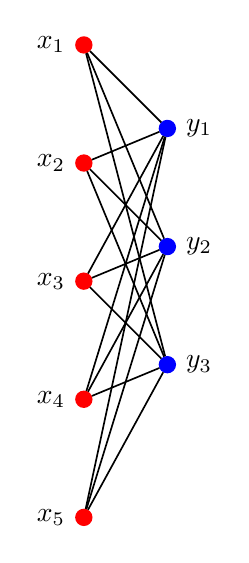
\begin{tikzpicture}[scale=.7,-,auto,node distance=1.5cm, semithick]
 				 		\tikzstyle{vert}=[draw, circle, inner sep=2pt,fill]
						\node[vert, color=blue, label=right:$y_1$]  (A) {};
							\node[vert, color=blue, label=right:$y_2$]  (B) [below of=A]{};
							\node[vert, color=blue, label=right:$y_3$]  (C) [below of=B]{};
							\node[vert, color=red, label=left:$x_1$]  (1) [above left of=A]{};
							\node[vert, color=red, label=left:$x_2$]  (2) [below of=1]{};		
							\node[vert, color=red, label=left:$x_3$]  (3) [below of=2]{};
		 					\node[vert, color=red, label=left:$x_4$]  (4) [below of=3]{};
		 					\node[vert, color=red, label=left:$x_5$]  (5) [below of=4]{};
		 				
		 					\foreach \i in {A,...,C}{
		 		 				\foreach \j in {1,...,5}{
		 							\draw  (\i) -- (\j);
		 						}
		 					}
 					\end{tikzpicture}
					\caption{$K_{5,3}$}		
					\label{fig_7_1}
				\end{figure}
				\item[iii] the graph of the octahedron.\\ {\color{black} \underline{Ans.} "\emph{Hamiltonian}", in fact all Platonic graphs are Hamiltonian} 
				\item[iv] the wheel $W_6$.\\ {\color{black} \underline{Ans.} "\emph{Hamiltonian}, as we can easily get a path that passing through all vertices exactly once."} 
				\item[v] the 4-cube $Q_4$.\\ {\color{black} \underline{Ans.} "\emph{Hamiltonian}, as shown in figure \ref{fig_5c_cube}, we can see that $|V(Q_4)| = 16$, while $\rho(\nu) = 4, \forall \nu \in V(Q_4)$}. 
			\end{itemize}
			}
			\hsplit
	\item[(7b)] {\color{blue}
			\begin{itemize}
				\item[i] For which values of $n$ is $K_n$ Hamiltonian? \\ {\color{black} \underline{Ans.} If $n=2$.}
				\item[ii] Which complete bipartite graphs are Hamiltonian?\\ {\color{black} \underline{Ans.} All $K_{n,n}$.} 
				\item[iii] Which Platonic graphs are Hamiltonian?\\ {\color{black} \underline{Ans.} All Platonic graphs} 
				\item[iv] For which values of $n$ is the wheel $W_n$ Hamiltonian?\\ {\color{black} \underline{Ans.} All Wheels.} 

				\item[v] For which values of $k$ if the $k-$cube $Q_n$ Hamiltonian?
			\end{itemize}	
			}
\end{itemize}

\section*{Some applications}
\begin{itemize}
		\item The short path problem.
		\item The Chinese postman problem.
		\item The travelling salesman problem.
\end{itemize}

\section*{9: Elementary properties of trees}
\begin{itemize}
		\item A \textbf{forest} is defined to be a graph which contains no cycles and a connected forest is called a \textbf{\emph{tree}}.
		\item \underline{\emph{\color{magenta} Theorem 9A}} \emph{Let $T$ be a graph with $n$ vertices. Then the following statements are equivalent:
			\begin{itemize}
				\item[(i)] $T$ is a tree.
				\item[(ii)] $T$ contains no cycles, and has $n-1$ edges.
				\item[(iii)] $T$ is connected, and has $n-1$ edges.
				\item[(iv)] $T$ is connected, and every edge is a bridge.
				\item[(v)] any two vertices of $T$ are connected by exactly one path.
				\item[(vi)] $T$ contains no cycles, but the addition of any new edge creates exactly one cycle.
			\end{itemize}
				} 
		\item \underline{\emph{\color{magenta} Corollary 9B}} \emph{If $G$ be a forest with $n$ vertices and $k$ components, then $G$ has $n-k$ edges.}
\item \begin{small} Given any connected graph $G$, we can choose a cycle and remove any one of its edges, and the resulting graph remains connected. If we repeat this procedure until there are no cycles left. The graph that remains is a tree that connects all the vertices of $G$. It is called a \underline{\emph{\color{magenta} spanning tree}} of $G$. Generally, if $G$ is an arbitrary graph with $n$ vertices, $m$ edges and $k$ components, then we can carry out this procedure on each component of $G$. The result is	called a \underline{\emph{\color{magenta} spanning forest}}, and the total number of edges removed in this process is the \underline{\emph{\color{magenta} cycle rank}} of $G$, denoted by $\gamma(G) = m - n + k$. the cutset rank of $G$ to be the number of edges in a spanning forest, denoted by $\xi(G) = n - k$ \end{small}
		\item \underline{\emph{\color{magenta} Theorem 9C}} \emph{If $T$ is any spanning forest of a graph $G$, then
			\begin{itemize}
				\item[(i)] every cutset of $G$ has an edge in common with $T$.
				\item[(ii)] every cutset of $G$ has an edge in common with the complement of $T$.
			\end{itemize}
		}
		\item For $T$ and $G$ in last theorem, if we add to $T$ any edge of $G$ not contained in $T$, then by statment ($vi$) in theorem (9A) we get a unique cycle. The set of all cycles formed in this way is called \underline{\emph{\color{magenta} fundamental set of cycles}} associated with $T$. Note, if $T$ is spanning tree of $G$, then the \emph{fundamental set of cycles} of $T$ is equal to \emph{cycle rank} of $G$.
\end{itemize}

\section*{Exercise 9}
	\begin{itemize}
		\item {\color{blue} Prove that every tree is a bipartie graph.}\\
			Let's first investigate the following example:
			\begin{figure}[h!]
				\centering
				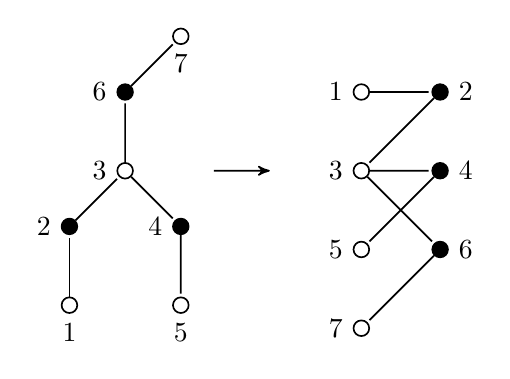
\begin{tikzpicture}[scale=0.3,-,>=stealth',shorten >=1pt, auto, node distance=1cm, semithick]
					\tikzstyle{vert}=[draw, circle, inner sep=2pt]
					\node[vert,label=below:1] (a1)	{};
					\node[vert,fill=black,label=left:2] (a2)	[above of=a1]{};
					\node[vert,label=left:3] (a3)	[above right of=a2]{};
					\node[vert,fill=black,label=left:4] (a4)	[below right of=a3]{};
					\node[vert,label=below:5] (a5)	[below of=a4]{};
					\node[vert,fill=black,label=left:6] (a6)	[above of=a3]{};
					\node[vert,label=below:7] (a7)	[above right of=a6]{};

					\node (c1) [right of=a3] {};
					\node (c2) [right of=c1] {};

					\node[vert,label=left:3] (b3)	[right of=c2]{};
					\node[vert,label=left:1] (b1)	[above of=b3]{};
					\node[vert,fill=black,label=right:2] (b2)	[right of=b1]{};
					\node[vert,fill=black,label=right:4] (b4)	[below of=b2]{};
					\node[vert,label=left:5] (b5)	[below of=b3]{};
					\node[vert,fill=black,label=right:6] (b6)	[below of=b4]{};
					\node[vert,label=left:7] (b7)	[below of=b5]{};

					\draw[->] (c1) -- (c2);
					\path
						(a1) edge (a2) 
						(a2) edge (a3) 
						(a3) edge (a4) 
						(a4) edge (a5)
						(a3) edge (a6)
						(a6) edge (a7)
						
						(b1) edge (b2) 
						(b2) edge (b3) 
						(b3) edge (b4) 
						(b4) edge (b5)
						(b3) edge (b6)
						(b6) edge (b7);
				\end{tikzpicture}
				\caption{Example, shows how a tree can be treated as a bipartite graph}
			\end{figure}
			with the aid of the example demonstrated in the last figure, we can formulate this property,
			\begin{eqnarray*}
					\forall u,v,w &\in& V(G),\\ 
					\text{if } \exists vw, uv &\in& E(G), \text{then } vw \not\in E(G),
			\end{eqnarray*}
			vthat is, for any tree, we can construct two sets/components $x,y$ where there are only edges between vertices from $x$ to vertices from $y$. (definition of bipartite graph)
			\item {\color{blue} Which trees are complete bipartite graphs?}
				It is easily to show that $K_{1,n}$, where $n \geq 2$ is a tree and a complete bipartite graph in the same time as shown in the next figure, but $K_{2,2}$ does not, as it has a cycle between its edges, as shown in the same figure,

				\begin{figure}[h!]
				\centering
				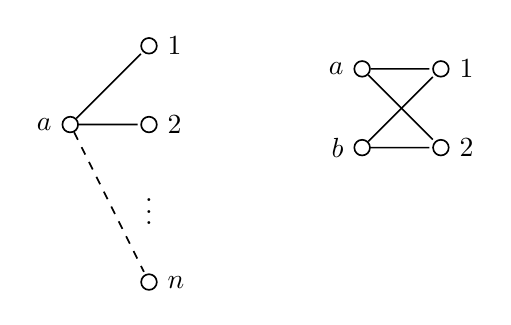
\begin{tikzpicture}[scale=0.3,-,>=stealth',shorten >=1pt, auto, node distance=1cm, semithick]
					\tikzstyle{vert}=[draw, circle, inner sep=2pt]
					\node[vert,label=right:1] (a1)	{};
					\node[vert,label=right:2] (a2)	[below of=a1]{};
					\node (a3)	[below of=a2]{$\vdots$};
					\node[vert,label=right:$n$] (an)	[below of=a3]{};
					\node[vert,label=left:$a$] (a) [left of=a2]{};
					\draw[dashed] (a) -- (an);
					
					\node (c1) [right of=a2] {};
					\node (c2) [right of=c1] {};

					\node[vert,label=left:$a$] (b1) [above right of=c2]{};
					\node[vert,label=left:$b$] (b2) [below of=b1]{};
					\node[vert,label=right:$1$] (1) [right of=b1]{};
					\node[vert,label=right:$2$] (2) [below of=1]{};
					\path
						(a) edge (a1)
						(a) edge (a2)
						(b1) edge (1) edge (2)
						(b2) edge (1) edge (2);
				\end{tikzpicture}
				\caption{$K_{1,n}, n \geq 2$ is a tree, but not $K_{m,n}, m,n \geq 2$}
			\end{figure}
			and in fact, we can embed $K_{2,2}$ in any $K_{m,n}, m,n \geq 2$. That is, our conculsion in the last figure caption.


		\item {\color{blue} Draw all the spanning trees in the graph of the following figure}.
			\begin{figure}[h!]
				\centering
				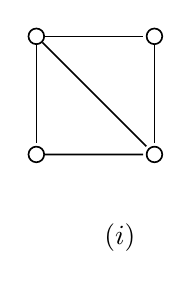
\begin{tikzpicture}[scale=.3,-,>=stealth',shorten >=1pt,auto,node distance=1.5cm, semithick]
						\tikzstyle{vert}=[draw, circle, inner sep=2pt]
						\node[vert] 		(A)                    		{};
 					 	\node[vert] 			(B) [below of=A]            {};
 					 	\node[vert] 			(C) [right of=B]            	{};
 					 	\node[vert] 			(D) [right of=A]            {};
						\node [below right of=B]		{($i$)};
 				  \path
					 (A) edge (B)
			 		 (A) edge (D)
					 (A) edge (C)
					 (D) edge (C)
					 (B) edge (C);
				\end{tikzpicture}		
				\qquad
				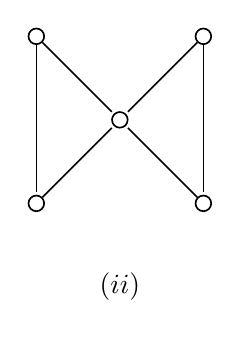
\begin{tikzpicture}[scale=.3,-,>=stealth',shorten >=1pt,auto,node distance=1.5cm, semithick]
						\tikzstyle{vert}=[draw, circle, inner sep=2pt]
						\node[vert] 		(C)                    		{};
 					 	\node[vert] 			(A) [above left of=C]            {};
						\node[vert] 			(D) [above right of=C]            	{};
						\node[vert] 			(E) [below right of=C]            {};
 					 	\node[vert] 			(B) [below left of=C]            {};
						\node [below right of=B]		{($ii$)};
 				  \path
					 (A) edge (C)
			 		 (A) edge (B)
					 (D) edge (C)
					 (D) edge (E)
					 (B) edge (C)
					 (E) edge (C);
				\end{tikzpicture}
			\end{figure} \\
			\underline{Ans.} of ($i$)
			\begin{figure}[h!]
				\centering
				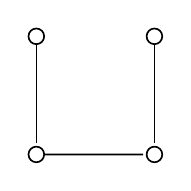
\begin{tikzpicture}[scale=.3,-,>=stealth',shorten >=1pt,auto,node distance=1.5cm, semithick]
						\tikzstyle{vert}=[draw, circle, inner sep=2pt]
						\node[vert] 		(A)                    		{};
 					 	\node[vert] 			(B) [below of=A]            {};
 					 	\node[vert] 			(C) [right of=B]            	{};
 					 	\node[vert] 			(D) [right of=A]            {};
 				  \path
					 (A) edge (B)
			 		 %(A) edge (D)
					 %(A) edge (C)
					 (D) edge (C)
					 (B) edge (C);
				\end{tikzpicture}		
				\qquad
				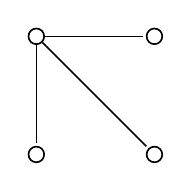
\begin{tikzpicture}[scale=.3,-,>=stealth',shorten >=1pt,auto,node distance=1.5cm, semithick]
						\tikzstyle{vert}=[draw, circle, inner sep=2pt]
						\node[vert] 		(A)                    		{};
 					 	\node[vert] 			(B) [below of=A]            {};
 					 	\node[vert] 			(C) [right of=B]            	{};
 					 	\node[vert] 			(D) [right of=A]            {};
 				  \path
					 (A) edge (B)
			 		 (A) edge (D)
					 (A) edge (C);
					 %(D) edge (C)
					 %(B) edge (C);
				\end{tikzpicture}	
			\end{figure}\\
			\underline{Ans.} of ($ii$)
			\begin{figure}[h!]
			\centering	
			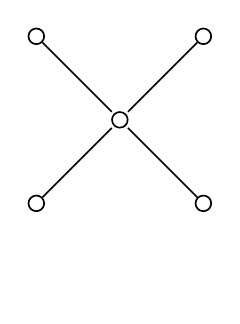
\begin{tikzpicture}[scale=.3,-,>=stealth',shorten >=1pt,auto,node distance=1.5cm, semithick]
						\tikzstyle{vert}=[draw, circle, inner sep=2pt]
						\node[vert] 		(C)                    		{};
 					 	\node[vert] 			(A) [above left of=C]            {};
						\node[vert] 			(D) [above right of=C]            	{};
						\node[vert] 			(E) [below right of=C]            {};
 					 	\node[vert] 			(B) [below left of=C]            {};
						\node [below right of=B]		{};
 				  \path
					 (A) edge (C)
			 		 %(A) edge (B)
					 (D) edge (C)
					 %(D) edge (E)
					 (B) edge (C)
					 (E) edge (C);
				\end{tikzpicture}
			\qquad
			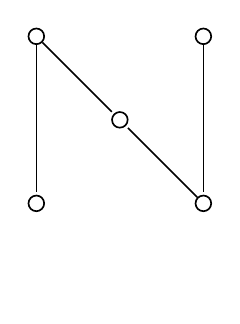
\begin{tikzpicture}[scale=.3,-,>=stealth',shorten >=1pt,auto,node distance=1.5cm, semithick]
						\tikzstyle{vert}=[draw, circle, inner sep=2pt]
						\node[vert] 		(C)                    		{};
 					 	\node[vert] 			(A) [above left of=C]            {};
						\node[vert] 			(D) [above right of=C]            	{};
						\node[vert] 			(E) [below right of=C]            {};
 					 	\node[vert] 			(B) [below left of=C]            {};
						\node [below right of=B]		{};
 				  \path
					 (A) edge (C)
			 		 (A) edge (B)
					 %(D) edge (C)
					 (D) edge (E)
					 %(B) edge (C)
					 (E) edge (C);
				\end{tikzpicture}
				\qquad
				\begin{tikzpicture}[scale=.3,-,>=stealth',shorten >=1pt,auto,node distance=1.5cm, semithick]
						\tikzstyle{vert}=[draw, circle, inner sep=2pt]
						\node[vert] 		(C)                    		{};
 					 	\node[vert] 			(A) [above left of=C]            {};
						\node[vert] 			(D) [above right of=C]            	{};
						\node[vert] 			(E) [below right of=C]            {};
 					 	\node[vert] 			(B) [below left of=C]            {};
						\node [below right of=B]		{};
 				  \path
					 (A) edge (C)
			 		 (A) edge (B)
					 (D) edge (C)
					 (D) edge (E)
					 %(B) edge (C)
					 %(E) edge (C);
				\end{tikzpicture}
				\qquad
				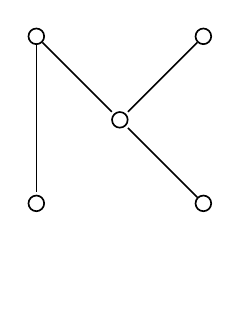
\begin{tikzpicture}[scale=.3,-,>=stealth',shorten >=1pt,auto,node distance=1.5cm, semithick]
						\tikzstyle{vert}=[draw, circle, inner sep=2pt]
						\node[vert] 		(C)                    		{};
 					 	\node[vert] 			(A) [above left of=C]            {};
						\node[vert] 			(D) [above right of=C]            	{};
						\node[vert] 			(E) [below right of=C]            {};
 					 	\node[vert] 			(B) [below left of=C]            {};
						\node [below right of=B]		{};
 				  \path
					 (A) edge (C)
			 		 (A) edge (B)
					 (D) edge (C)
					 %(D) edge (E)
					 %(B) edge (C)
					 (E) edge (C);
				\end{tikzpicture}
	

			\end{figure}
	\item {\color{blue} Find the fundamental sets of cycles and cutsets of the graph if the following figure, associated with the spanning tree shown}
					\begin{figure}[h!]
					\centering
					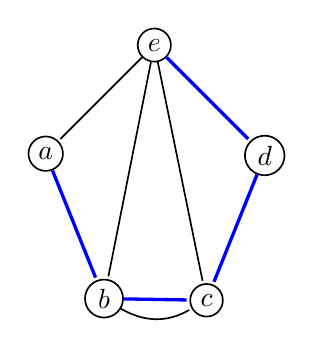
\begin{tikzpicture}[scale=.3,-,>=stealth',shorten >=1pt,auto,node distance=1.5cm, semithick]
						\tikzstyle{vert}=[draw, circle, inner sep=2pt]
						\node[vert] 		(E)                    		{$e$};
 					 	\node[vert] 			(A) [below left=1.5cm of E]            {$a$};
						\node[vert] 			(D) [below right=1.5cm of E]            	{$d$};
						\node[vert] 			(C) [below left=1.5cm and 0.4cm of D]            {$c$};
 					 	\node[vert] 			(B) [below right=1.5cm and 0.4cm of A]            {$b$};
				
						\path
							(E) edge (A)
							(E) edge [very thick, blue] (D)
							(A) edge [very thick, blue] (B)
							(D) edge [very thick, blue] (C)
							(B) edge [very thick, blue] (C)
							(B) edge [bend right] (C)
							(E) edge (B)
							(E) edge (C);

				\end{tikzpicture}	
				\end{figure}\\
				\underline{Ans.} 
				\begin{figure}[h!]
					\centering
					\begin{tikzpicture}[scale=.2,-,>=stealth',shorten >=1pt,auto,node distance=1.5cm, semithick]
						\tikzstyle{vert}=[draw, circle, inner sep=2pt]
						\node[vert] 		(E)                    		{};
 					 	\node[vert] 			(A) [below left=1.5cm of E]            {};
						\node[vert] 			(D) [below right=1.5cm of E]            	{};
						\node[vert] 			(C) [below left=1.5cm and 0.4cm of D]            {};
 					 	\node[vert] 			(B) [below right=1.5cm and 0.4cm of A]            {};
				
						\path
							(E) edge [red] (A)
							(E) edge [very thick, blue] (D)
							(A) edge [very thick, blue] (B)
							(D) edge [very thick, blue] (C)
							(B) edge [very thick, blue] (C)
							%(B) edge [bend right] (C)
							%(E) edge (B)
							%(E) edge (C);
				\end{tikzpicture}
				\qquad
				\begin{tikzpicture}[scale=.2,-,>=stealth',shorten >=1pt,auto,node distance=1.5cm, semithick]
						\tikzstyle{vert}=[draw, circle, inner sep=2pt]
						\node[vert] 		(E)                    		{};
 					 	\node[vert] 			(A) [below left=1.5cm of E]            {};
						\node[vert] 			(D) [below right=1.5cm of E]            	{};
						\node[vert] 			(C) [below left=1.5cm and 0.4cm of D]            {};
 					 	\node[vert] 			(B) [below right=1.5cm and 0.4cm of A]            {};
				
						\path
							%(E) edge [red] (A)
							(E) edge [very thick, blue] (D)
							(A) edge [very thick, blue] (B)
							(D) edge [very thick, blue] (C)
							(B) edge [very thick, blue] (C)
							(B) edge [bend right, red] (C)
							%(E) edge (B)
							%(E) edge (C);
				\end{tikzpicture}
				\qquad
				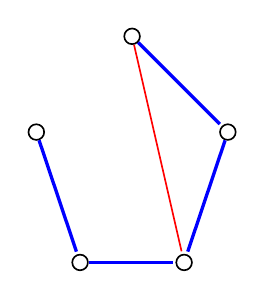
\begin{tikzpicture}[scale=.2,-,>=stealth',shorten >=1pt,auto,node distance=1.5cm, semithick]
						\tikzstyle{vert}=[draw, circle, inner sep=2pt]
						\node[vert] 		(E)                    		{};
 					 	\node[vert] 			(A) [below left=1.5cm of E]            {};
						\node[vert] 			(D) [below right=1.5cm of E]            	{};
						\node[vert] 			(C) [below left=1.5cm and 0.4cm of D]            {};
 					 	\node[vert] 			(B) [below right=1.5cm and 0.4cm of A]            {};
				
						\path
							%(E) edge [red] (A)
							(E) edge [very thick, blue] (D)
							(A) edge [very thick, blue] (B)
							(D) edge [very thick, blue] (C)
							(B) edge [very thick, blue] (C)
							%(B) edge [bend right, red] (C)
							%(E) edge [red] (B)
							(E) edge [red] (C);
				\end{tikzpicture}

				\end{figure}

	\end{itemize}
	
\section*{10: The enumeration of trees}
\begin{itemize}
	\item \underline{\emph{\color{magenta} Labelling}} of a graph $G$ on $n$ vertices to be one-one mapping from the vertex-set of $G$ onto the set ${1, \cdots ,n}$, a \underline{\emph{\color{magenta} labelled graph}} is then a pair $(G, \phi)$, where $\phi$ is a labelling of $G$.
	\item \underline{\emph{\color{magenta}Theorem 10A} (Cayley)} \hl{\emph{There are $n^{n-2}$ distinct labelled trees on $n$ vertices}}.
	\item \underline{\emph{\color{magenta}Corrollary 10B}} \emph{The number of spanning trees of $K_n$ is $n^{n-2}$}.
	\item \underline{\emph{\color{magenta}Theorem 10C}} \emph{Let $G$ be a connected simple graph with vertex set $\{v_1,\cdots,v_n \}$, and let \textbf{M} $= (m_{ij})$ be $n \times n$ matrix in which $m_{ii} = \rho(v_i), m_{ij} = -1 $ if $v_i$ and $v_j$ are adjacent, and $m_{ij}=0$ otherwise. Then the number of spanning trees of $G$ is equal to the cofactor of any element of \textbf{M}}.	
\end{itemize}

\section*{Exercise 10}
\begin{itemize}
	\item {\color{blue} Verify directly that there are exactly 125 labelled trees on five vertices.}
	\item {\color{blue} \begin{itemize}
		\item[(i)] Show that there are exactly $2^{n(n-1)/2}$ labelled simple graphs on $n$ vertices.
		\item[(ii)] How many of these have exactly $m$ edges?
	\end{itemize}}
	\item {\color{blue} In the first proof of Cayley's theorem, fin:
	\begin{itemize}
			\item[(i)] the labelled trees corresponding to the sequences (1,2,3,4) and (3,3,3,3).
		\item[(ii)] the sequences corresponding to the labelled tree in the following figure
	\end{itemize}}
	\begin{figure}[h!]
				\centering
				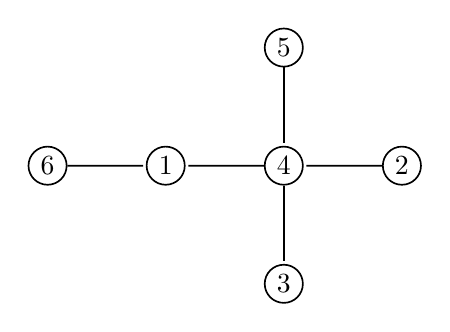
\begin{tikzpicture}[scale=.3,-,>=stealth',shorten >=1pt,auto,node distance=1.5cm, semithick]
						\tikzstyle{vert}=[draw, circle, inner sep=2pt]
						\node[vert] 		(5)                    		{$5$};
						\node[vert] 			(4) [below of=5]            {$4$};
 					 	\node[vert] 			(2) [right of=4]            	{$2$};
 					 	\node[vert] 			(1) [left of=4]            {$1$};
 					 	\node[vert] 			(6) [left of=1]            {$6$};
 					 	\node[vert] 			(3) [below of=4]            {$3$};
 				  \path
					 (5) edge (4)
			 		 (4) edge (3)
					 (2) edge (4)
					 (4) edge (1)
					 (6) edge (1);
				\end{tikzpicture}	

				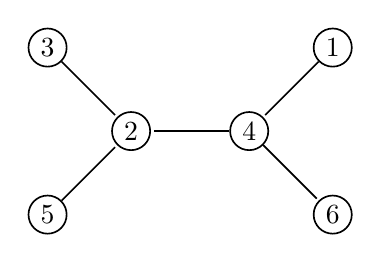
\begin{tikzpicture}[scale=.3,-,>=stealth',shorten >=1pt,auto,node distance=1.5cm, semithick]
						\tikzstyle{vert}=[draw, circle, inner sep=2pt]
						\node[vert] 		(2)                    		{$2$};
						\node[vert] 			(4) [right of=2]            {$4$};
 					 	\node[vert] 			(3) [above left of=2]            	{$3$};
 					 	\node[vert] 			(1) [above right of=4]            {$1$};
 					 	\node[vert] 			(6) [below right of=4]            {$6$};
 					 	\node[vert] 			(5) [below left of=2]            {$5$};
 				  \path
					 (5) edge (2)
			 		 (4) edge (2)
					 (1) edge (4)
					 (4) edge (6)
					 (3) edge (2);
				\end{tikzpicture}	
			\end{figure}
	\item {\color{blue} How many spanning trees has $K_{2,s}$?}
\end{itemize}

\section*{More Applications}
\begin{itemize}
	\item The minimum connector problem.
	\item Enumeration of chemical molecules.
	\item Electrical networks.
\end{itemize}

\section*{12: Planar graphs}
\begin{itemize}
		\item A \underline{\emph{\color{magenta} plane graph}} is a graph drawn in the plane in such a way that no two edges intersect geometrically except at a vertex to which they are both incident. \begin{small} a planar graph is one which is isomorphic to a plane graph.\end{small}
				\item \underline{\emph{\color{magenta} Theorem 12A}}: \emph{\hl{$K_5$, and $K_{3,3}$ are non-planer}}
				\item Two graphs are \underline{\emph{\color{magenta} homomorphic}} if they can both be obtained from the same graph by inserting new vertices of degree two into its edges.
				\item \underline{\emph{\color{magenta} Theorem 12B}}: \emph{A graph is \hl{planar} iff it contains \hl{no subgraph homeomorphic to $K_5$, and $K_{3,3}$}}
				\item \underline{\emph{\color{magenta} Theorem 12C}}: \emph{A graph is \hl{planar} iff it contains \hl{no subgraph which contractible to $K_5$, and $K_{3,3}$}}


\end{itemize}
\section*{Exercise 12}
\begin{itemize}
	\item[(12c)] {\color{blue}Prove that the Petersen graph is non-planar
					\begin{itemize}
							\item[(i)] by using Theorem 12B,
							\item[(ii)] by using Theorem 12C.
						\end{itemize}
			}
	\item[(12d)] {\color{blue} Give an example of
					\begin{itemize}
						\item[(i)] a non-planar graph which is not homeomorphic to $K_5$ or $K_{3,3}$,
						\item[(ii)] a non-planar graph which is not contractible to $K_5$ or $K_{3,3}$.								
					\end{itemize}
					Why does the existence of these graphs not contradict Theorems 12B and 12C?
			
			}
\end{itemize}
\section*{13: Euler's formula for plane graphs}
\begin{itemize}
		\item If $x$ is a point of the plane disjoint from $G$, the \underline{\emph{\color{magenta}face}} of $(G)$ \underline{\emph{color{magenta}containing $x$}} is the set of all points of the plane which can be reached from $x$ by a Jordan curve all of whose points are disjoint from $G$.
		\item \underline{\emph{\color{magenta}Theorem 13A (Euler)}}: Let $G$ be a connected plane graph, and let $n, m$ and $f$ denote respectively the number of vertices, edges and faces of $G$, then \hl{$n - m + f = 2$}.
		\item \underline{\emph{\color{magenta}Corollary 13B}}: \emph{let $G$ be a \hl{polyhedral} graph, then with above notation \hl{$n - m + f = 2$}}.
		\item \underline{\emph{\color{magenta}Corollary 13C}}: \emph{let $G$ be a \hl{plane} graph with $n$ vertices, $m$ edges, $f$ faces and $k$ components, then \hl{$n - m + f = k + 1$}}.
		\item \underline{\emph{\color{magenta}Corollary 13D}}: \emph{(i) If $G$ is a connected simple planar graph with $n(\geq 3)$ vertices and $m$ edges, then $m \leq 3n -6$}\\ (ii) If, in addition, $G$ has no triangles, then $m \leq 2n -4$.
		\item \underline{\emph{\color{magenta}Corollary 13E}}: \emph{$K_5$ and $K_{3,3}$ are non-planar}.
		\item \underline{\emph{\color{magenta}Corollary 13F}}: \emph{Every simple planar graph contains a vertex whose degree is at most five}.
		\item The \underline{\emph{\color{magenta}thickness}} of a graph $t(G)$ is the smallest number of planar graphs which can be superimposed to form $G$.
		\item \underline{\emph{\color{magenta}Theorem 13G}}: \emph{Let $G$ be a simple graph with $n(\geq 3)$ vertices and $m$ edges, then the thickness $t(G)$ of $G$ satisfies the following inequalities:
						$$t(G) \geq \big \lceil \frac{m}{3n -6} \big \rceil; \ \ \ \ \ t(G) \geq \big \lfloor \frac{m + 3n -7}{3n -6} \big \rfloor $$
				}		
\end{itemize}
\section*{Exercise 13}
\begin{itemize}
	\item[(13c)] {\color{blue}
			\begin{itemize}
				\item[(i)] Use Euler's formula to prove that if $G$ is a connected plane graph of girth 5 then, with the above notation, $m \leq \frac{5}{3} (n-2)$.
				\item[(ii)] Deduce the Petersen graph is non-planar.
				\item[(iii)] Obtain an inequality, generalizing that in part (i), for connected plane graphs of girth $r$.
			\end{itemize}
	}
	\item[(13h)] {\color{blue} Find the thickness of
			\begin{itemize}
				\item[(i)] the Petersen graph.
				\item[(ii)] the 4-cube $Q_4$.
			\end{itemize}
			}
\end{itemize}

\section*{14: Graphs on other surfaces}

\section*{Exercise 14}

\section*{15: Dual graphs}
\begin{itemize}
	\item \underline{\emph{\color{magenta}Geometric-dual $G^*$}} of graph $G$ constructed as follows:
			\begin{itemize}
				\item[(i)] inside each face $F_i$ of $G$ we choose a point $v_i^*$ --- these points are the vertices of $G^*$,
				\item[(ii)] corresponding to each edge $e$ of $G$ we draw a line $e^*$ which crosses $e$ (but no other edge of $G$), and joins the vertices $v_i^*$ which lie in the faces $F_i$ adjoining $e$ --- these lines are the edges of $G^*$.
			\end{itemize}
	\item \underline{\emph{\color{magenta}Lemma 15A}}: \emph{Let $G$ be a plane connected graph with $n$ vertices, $m$ edges and $f$ faces, and let its geometric-dual $G^*$ have $n^*$ vetices. $m^*$ edges and $f^*$ faces. Then $n^* = f, m^* = m, \text{and} f^* = n$}.
	\item \underline{\emph{\color{magenta}Theorem 15B}}: \emph{\hl{Let $G$ be a plane connected graph. Then $G^{**}$ is isomorphic to $G$}}.
	\item \underline{\emph{\color{magenta}Theorem 15C}}: \emph{\hl{Let $G$ be a planar and $G^*$ be a geometric-dual of $G$. Then a set of edges in $G$ forms a cycle in $G$ iff the corresponding set of edges of $G^*$ forms a cutset in $G^*$}}.
	\item \underline{\emph{\color{magenta}Corollary 15D}}: \emph{A set of edges of $G$ forms a cutset in $G$ iff the corresponding set of edges of $G^*$ forms a cycle in $G^*$.
	\item The \underline{\emph{\color{magenta}abstract-dual}} $G^*$ of a graph $G$ if there is a one-one correspondance between the edges of $G$ and those of $G^*$ with the property that a set of edges of $G$ forms a cycle in $G$ iff the corresponding set of edges of $G^*$ forms a cutset in $G^*$}.
	\item \underline{\emph{\color{magenta}Theorem 15E}}: \emph{\hl{If $G^*$ is an abstact-dual of $G$, then $G$ is an abstact-dual of $G^*$}}.
	\item \underline{\emph{\color{magenta}Theorem 15F}}: \emph{\hl{A graph is planar iff it has an abstract-dual}}.
\end{itemize}
\section*{Exercise 15}

\section*{16: Infinite graphs}

\section*{Exercise 16}


\end{document}

